\documentclass[10pt]{article}

% Packages
\usepackage{enumerate}
\usepackage{mathptmx}
\usepackage{hyperref}
\usepackage{helvet}
\usepackage{listings}
\usepackage[left=0.75in,right=0.75in,top=0.875in,bottom=0.875in]{geometry}
\usepackage{titling}
\usepackage{tabularx}
\usepackage{multicol}
\usepackage[explicit]{titlesec}
\usepackage{graphicx}
\usepackage{xcolor}

% Single column figure
\newenvironment{InlineColumnFigure}
{\par\medskip\noindent\minipage{\linewidth}}
{\endminipage\par\medskip}

% Caption
\newcommand{\Caption}[1]
{\vspace{0mm}\fontsize{9}{9}\textbf{Figure \refstepcounter{figCounter} 
\arabic{figCounter}: #1}}

\newcounter{figCounter}
\setcounter{figCounter}{0}

% ACM CHI Format
\setlength{\columnsep}{0.85cm}
\setlength{\parindent}{0pt}

\titlespacing{\section}{0pt}{10pt}{-\parskip}
\titlespacing{\subsection}{0pt}{10pt}{-\parskip}
\titlespacing{\subsubsection}{0pt}{10pt}{-\parskip}

\titleformat{\section}{\normalfont\fontsize{9}{9}\sffamily\bfseries}
{\thesection}{1em}{\MakeUppercase{#1}}
\titleformat{\subsection}{\normalfont\fontsize{9}{9}\sffamily\bfseries}
{\thesubsection}{1em}{#1}
\titleformat{\subsubsection}{\normalfont\fontsize{9}{9}\sffamily\itshape}
{\thesubsubsection}{1em}{#1}

\pagenumbering{gobble}

%===============================- 80 columns -=================================%
\begin{document}

% Title
\begin{center}
{\LARGE \sffamily \textbf{Course-Management System: Final Report} 
\vspace{2mm}}\\
\begin{tabular}{cccc}
\textbf{Stuart Douglas} & \textbf{Matthew Pagnan} & \textbf{Rob Gorrie} & 
\textbf{Derek Dagworthy}\\
1214422 & 1208693 & 1222547 & 1214937\\
McMaster University & McMaster University & McMaster University & McMaster 
University\\
dougls2@mcmaster.ca & pagnanmm@mcmaster.ca & gorrierw@mcmaster.ca & 
dagwordj@mcmaster.ca\\
\end{tabular}
\end{center}
\vspace{2mm}

\begin{multicols}{2}

% =================== Section =================== 
\section*{Abstract}
The final report for a design project for a course-management system is presented 
here. The proposed course-management system allows university students to enroll in courses, view their 
schedule and perform other course-related tasks from a web portal.\\

Firstly, the proposed project and suggested improvements over existing systems are explained. To inform this, four Canadian university course-management systems were surveyed, and the surveys are presented after the suggested improvements. Each survey 
has a brief description of the software followed by a critique of the major usability flaws and 
strengths. Three personas are then presented to demonstrate the potential users of the system that guided the design process. Following personas, information about the usablily 
tests conducted for this system is presented followed by the results, discussion about the results, and final conclusions about the project.

\section*{Note about Formatting}
This document strictly follows the ACM CHI format. Extra spacing between paragraphs is created by LaTeX to better arrange content, and is not directly controllable by the creator. The format used for the Personas section is based off of the format given along with Milestone 2 to fit into the 2-column layout, with images included inline (which does not violate the ACM CHI template). Extreme care has been given to follow the specified format exactly, including fonts, margins, and figures.

% =================== Section =================== %
\section*{Introduction}

% =================== SubSection ================== %
The project proposed in this document is the design of a new 
university course-management system. Through scrutinization of several 
pre-existing systems, we will apply design concepts discussed in class to 
determine what features and design choices are crucial to the success of a course-
management system's design.\\

Users of the proposed system should be able to perform the following functions:
\begin{itemize}
\item enroll in courses
\item change timeslots for lectures, tutorials, and labs of enrolled courses
\item view weekly schedule
\item view exam schedule
\end{itemize}

In the following section we will introduce several possible improvements that 
could be made to existing systems, informed by the system surveys conducted. These suggested improvements were incorporated into designs mockups for the new system, and into the final design of the working system.

% =================== SubSection =================== %
\subsection*{Suggested Improvements to Existing Systems}
We have outlined several improvements over existing systems that have been incorporated into the design of the new system. The software surveys identified 
several key areas of weaknesses, and solutions to those are presented below.

\subsubsection*{Dynamic Element}
One of the highlighted points of weakness in all the systems surveyed was the 
ability to surface the most relevant data to the user quickly and consistently. 
To improve this aspect, the concept of an intelligent, ``dynamic'' element was 
proposed. This prominent element is the first thing users see on the home page of the enew system. Several factors including the current date and enrollment 
status are used to determine which task the user is most likely to perform.\\

For example, when the user accesses the system during exam season, the element 
 displays the student's exam schedule. During the course registration period, 
the element displays information related to course registration. If a user 
is not yet accepted into University, the element displays their application 
status.\\

This dynamic element helps users quickly find the information they are 
looking for by making information more visible and easier to access. All functions continue to be 
displayed below in a static and consistent manner, in case the user wishes to perform a less common task.

\subsubsection*{Improved Navigation}
Many tasks performed by users of course-management software are broken into 
several steps. A weakness of the existing products was in visually showing the 
user at which step they were at. To solve this, a ``breadcrumbs'' navigation element was added  when the user is engaged in a multi-step task. This element shows which step the user is currently on, and includes the ability to 
go back to a previous step, or jump ahead to the first uncompleted step.\\

This visual indicator improves the user's comprehension of how the system 
works, and gives them the ability to better navigate between steps. It also improves user satisfaction, 
as they are less likely to become impatient when they know exactly 
how many steps they have completed and how many remain. 

\subsubsection*{Smarter Schedule Generation}
An initial proposal for the system was to have the system generate several possibly schedules based on the users wishlist, and rank them based on several factors such as early classes, gaps between classes and having certain days completely off. We do believe this would be a meaningful addition to a course-management system, however decided not to include it in the final product due to time and resource constraints.

% =================== Section =================== %
\section*{Related Work}
Four course-management systems from Canadian universities were selected for 
review. For each system, a brief description was followed by a critique of 
the major usability flaws and strengths. From this, the main goals and tasks of 
users using the systems was extracted. 

% =================== SubSection =================== %
\subsection*{McMaster University -- Mosaic}
The purpose of the software is to allow students to manage their courses 
(enrolling, dropping etc.), and view information about their current status 
(current timetable, enrollment status, financial balance etc.). The main 
interface for the software consists of several collapsible modules 
encapsulating different aspects of the software in a main column. These include 
Academics, Finances, Personal Information, and Admissions. A small column to 
the right holds less common sections, such as Enrollment Dates and Graduation. 
The focus of this analysis is on two common tasks -- enrolling in courses and 
viewing one's course schedule.

\subsubsection*{Critique}
The largest usability flaws in Mosaic center around difficulty to access 
required information. Combined with an unintuitive and inconsistent navigation 
interface. The HTA for enrolling in a course (appendix: Figure 4) demonstrates this 
through the large number of steps required to perform a routine and common task. 
Other functions are hidden behind dropdown menus, and are difficult to discover.\\

The navigation is separated into a top navigation bar separated by user-type 
(e.g. Students and Employees). Within the student center page, functions are 
separated into modules, an effective strategy to group related functions. 
Navigating to one of the sub-functions (such as enrolling in a course) presents 
secondary and tertiary menus below the main one. Navigation within one of these 
is handled by blue text hyperlinks back to previous pages. Native back and 
forward browser functionality does not work. There is little visual indication 
of where the user is beyond the navigation bars at the top, which do not go to a 
depth sufficient to cover all pages used when performing common actions, such as 
enrolling in a course.

% =================== SubSection =================== %
\subsection*{Guelph University -- WebAdvisor}
Guelph University's course enrollment software, WebAdvisor, provides a variety 
of functions for students to manage their courses. The student page interface 
contains two columns -- a main column with course-related news, and a righthand 
column with links to each of the functions (Register for Courses, View Schedule 
etc). These ``function'' pages are one column, and may contain several sub-pages 
as processes are broken into steps. Navigating between sub-pages is done using 
native browser back and forward buttons. If an error occurs, such as no courses 
found for specific search criteria, a large box is displayed with information 
about the error and the option to search for a solution.

\subsubsection*{Critique}
There are a variety of usability issues associated with \mbox{WebAdvisor} that 
could be improved upon, especially in the area of navigation. There are also 
certain strengths to the system as compared to others surveyed. The navigation 
issues largely stem from a lack of consistent navigation elements to show the 
user where they are. For example, when enrolling in a course there are several 
steps that must be completed (appendix: Figure 10). The user is not aware how many steps there are total, how many they 
have completed or how many remain. Another large usability issue is an 
inefficient use of space on the main page. The visibility of important functions 
is reduced by putting all functions in a small column to the right of the main 
content. This main content contains news items, such as exam period times and 
service outages, generally information that the user is less likely to need than 
the functions beside it.\\

WebAdvisor does do some things quite well from a usability perspective however. 
One of the most common tasks is enrolling in a course, and WebAdvisor has the 
most streamlined process of all universities surveyed. Although it is not always 
clear at which step the user is at as discussed above, the process is 
straightforward and contains much fewer steps than performing a similar task 
using a different system.

% =================== SubSection =================== %
\subsection*{Carleton University -- Central}
Central is the course-management system for Carleton University. It has a 
similar feature-set to the other systems surveyed. This includes allowing users 
to enroll in courses and view their schedule. The user interface for Central 
primarily is based on text links to different pages, with very little use of 
icons or colour. The main student page is a one-column list of text links to the 
various student-related categories of functions. A tab bar at the top lets the 
user switch between different sections of the system including Student Services 
and Employee Services.

\subsubsection*{Critique}
There are a large number of prominent usability flaws in Carleton University's 
course-management system. Visibility of common functions on the main 
page is very low, as a long list of hyperlinks contains all the categories (e.g. 
Registration, Student Records etc) requiring the user to read each one until 
they find the correct one. Once a category is selected, then another list of 
hyperlinks to each of the functions in that category is shown. 
Again, the user must read through each one until they find the desired function.\\

Another large usability flaw is the poor mapping between many actions. For 
example, when adding a course, the user first enters a course number into one of 
several (unlabeled) input boxes, and then they click the Submit button (appendix: 
figure 13). The submit button is aligned with other buttons for Class Search, 
which takes the user to a separate page, Reset, which undoes their changes, and 
Return to Worksheet which navigates the user to a page showing them their 
preferred courses. These buttons are not all related, and grouping them together 
may confuse the user.\\

Overall, Central is a relatively unintuitive system, requiring users to spend 
more time finding the information they need through poor mappings and a lack of 
a visual hierarchy.

% =================== SubSection =================== %
\subsection*{Waterloo University -- Quest}
The Quest system is designed to let students manage several aspects 
of their university enrollment, such as course management, financial inquiries, 
and contact information. Students can also sign up for a GO Bus pass, view their 
grades and transcript, and check the status of scholarships and other 
applications. The main page is broken up into 8 collapsible sections, 4 main 
sections (Academics, Finances, Personal Information, Admissions) with another four 
sections in a sidebar (Holds, Finance Information, Academic Information, Other 
Useful Links). The critique will focus on enrolling in courses and viewing a 
user's course schedule.

\subsubsection*{Critique}
Quest has some major usability issues when it comes to providing the user to 
information and functions they can use. The system is notorious for hiding 
options and menus from the user, requiring several screens of drill down menus 
before being able to access any meaningful options. The menus look unfinished or 
poorly formatted, and it is easy to become lost and confused while navigating 
the various pages. Navigation on the main page uses hyperlinked text, 
while traversing the deeper options is done using blue menu tabs. Native browser 
back and forward commands generally work as expected, which makes navigation a 
little more manageable. 

\section*{Personas}
Presented are the personas used to develop our design.These personas were based off of the \emph{Persona Template} as linked from the assignment outline from McMaster University, COMP SCI 4HC3 These personas were created to archetype the most common user types, and have been integral to developing a product that will satisfy all of them.\\

%%============================= Persona 1 ======================================%
\subsection*{Trevor Clark}
\begin{center}

\includegraphics[width=50mm]{images/Trevor.jpg}\\
\Caption{``When do classes start?"}
\end{center}

\begin{itemize}
\item Born: London, ON
\item Age: 22
\item 3rd Year Engineering Student at McMaster
\end{itemize}

Trevor is a third year Civil Engineering student at McMaster. He currently lives 10 minutes away from campus with some friends he met in first year. Trevor's parents are paying for his tuition and he has a student loan which he uses to pay for rent and food.\\

Trevor is unorganized and rarely goes to class. He also forgets to hand in assignments on time. Trevor is not a part of any clubs and prefers to spend his free time with his housemates playing video games.\\

Trevor has trouble remembering important dates, like his course selection or when his exams are. When he searches for information, he usually gives up after five minutes if he cannot find what he is looking for. Trevor would like it if the new course management system was quick and easy to use. He also would not mind it if certain information was made more accessible during certain times of the year (easy to see link to exam schedule around exam season).

%%============================= Persona 2 ======================================%
\subsection*{Candice Smith}
\begin{center}

\includegraphics[width=70mm]{images/Candice.jpg}\\
\Caption{``I don't know what electives I want to take for university next year"}
\end{center}
\begin{itemize}
\item Born: Oakville, ON
\item Age: 18
\item Grade 12 High School Student
\end{itemize}

Candice has been accepted to the chemistry program at McMaster. Candice currently lives at home with her parents and will be moving into residence in the fall. Her parents are paying for her tuition, but Candice is paying for her residence and meal plan. Candice works part time at the Fortinos in her home town to save up money so she can go to the movies whenever new movies come out.\\

Candice has done well in all of her classes in high school and is a part of several high school groups; such as the volleyball team, track and field team and the Harry Potter fan club.\\

Candice has several electives that she can take, but she cannot decide which ones to enrol in. She has heard that she can change courses during the first couple weeks of class and plans on doing that if she ends up changing her mind. Candice has already made a list of classes she would like to take in her first year and is waiting for the course registration to open up. Candice would like the new course management system to allow her to browse all the courses available to her and would like it if there were descriptions for each course that she could read before she registers.

%%============================= Persona 3 ======================================%
\subsection*{Adrian Lopez}
\begin{center}

\includegraphics[width=70mm]{images/Adrian.png}\\
\Caption{``I have a lot of new things to get used to in Canada"}
\end{center}

\begin{itemize}
\item Born: Mexico City, Mexico
\item Age: 20
\item 2nd Year Geography Student on Exchange to McMaster
\end{itemize}

Adrian is a geography student from Mexico on exchange at McMaster for the year. Adrian is living in a house 20 minutes away from campus with other students in the foreign exchange program. Adrian's tuition is being paid for by a grant he received for being a part of the foreign exchange program. His parents are giving him some money for rent and food but Adrian has to pay for some of it himself. Adrian is a hard working individual during the week and can be found in the Thode library between classes. Adrian likes to get all of his assignments done during the week so he can spend his weekend going to clubs with his housemates and friends.\\

Adrian is a part of the improv club which he regularly goes to. Adrian has chosen a light course load this year as he would like some time to experience Canada before he goes back to Mexico next September.\\

Since English is not Adrian's first language he sometimes has trouble reading and understanding websites that are primarily text, and he can get confused while navigating to the information he is looking for. Adrian would like it if the new course management system was easy to navigate and intuitive enough that he doesn't need to read an instruction manual to know how to use it.

% =============================== USABILITY =========================== %
\section*{Design Mockups}
Please refer to the 

% =============================== USABILITY =========================== %
\section*{Usability Tests}
\subsection*{Overview}
This section of the document describes a plan for conducting a usability test for our course management software. This usability test plan will be based off of the \href{http://www.usability.gov/how-to-and-tools/resources/templates/usability-test-plan-template.html}{\underline{Usability Test Plan Template}} created by the U.S. Department of Health \& Human Services. The goals of this usability test are to establish a baseline of user performance, establish and validate user performance measures, and identify potential design concerns to be addressed in order to improve the efficiency, productivity, and end-user satisfaction of the product.\\

The usability test objectives are:
\begin{itemize}
\item To determine design inconsistencies and usability problem areas within the user interface and content areas. 

	\begin{itemize}
	\item Navigation errors - failure to locate functions, failure to follow recommended screen flow.
	\item Presentation errors - failure to locate and properly act upon desired information in screens, selection errors due to 				labeling ambiguities
	\end{itemize}
	
\item Exercise the web site under controlled test conditions with representative users. Data will be used to access whether usability goals regarding an effective, efficient, and well-recieved user interface have been achieved.

\item Establish baseline user performance and user-satisfaction levels of the user interface for future usability evaluations.
\end{itemize}

\subsection*{Procedure}
The participant's interaction with the application will be monitored by the facilitator seated in the same room. The facilitator will be responsible for taking notes and logging data during the tests.
The facilitator will explain that the amount of time taken to complete the test task will be measured as well as how many errors were made. At the start of each task the facilitator will inform the participant of the tasks objective.\\

Once the participant starts the task the facilitator will begin to time the participant.  The facilitator will instruct the participant to `think aloud' so that verbal record exists of their interaction with the application. The facilitator will observe and enter user behavior, user comments, and system actions. After the participant has completed all tasks they will be asked to complete a questionnaire.\\

Following is a list of the tasks the participant will complete. The reason the courses in tasks 1.1 and 2.1 are different is that dummy courses were used for the new system, and have different course codes.
\begin{itemize}
\item \textbf{Task 1.1} - Have user enroll in the following courses for \emph{Winter 2016} through Mosaic, selecting lectures, tutorials, and sections so as to eliminate conflicts as needed:
\begin{itemize}
\item ANTHROP 1AA3
\item ANTHROP 1AB3
\item COMPSCI 2DM3
\item BIOLOGY 1A03
\end{itemize}
\item \textbf{Task 1.2} - Have user find their exam schedule for the Fall 2015 semester on Mosaic 
\item \textbf{Task 1.3} - Have user find their weekly schedule for the Fall 2015 semester on Mosaic
\item \textbf{Task 2.1} -  Have user enroll in the following courses using the new system selecting lectures, tutorials, and sections so as to eliminate conflicts as needed:
\begin{itemize}
\item ANTHROP 4AA3
\item ANTHROP 4M03
\item COMP SCI 1TA3
\item BIOLOGY 2AA3
\end{itemize}
\item \textbf{Task 2.2} - Have user find their exam schedule for the Fall 2015 semester using the new system
\item \textbf{Task 2.3} - Have user find their weekly schedule for the Fall 2015 semester using the new system
\end{itemize}

\subsection*{Usability Metrics}
Usability metrics refers to user performance measured against specific performance goals necessary to satisfy usability requirements. Scenario completion success rates, error rates, subjective evaluations, and scenario completion times will be used.\\

\subsubsection*{Scenario Completion}
Each scenario will require that the participant performs a specific, common task. The scenario is complete when the scenario's goal has been obtained or the participant requests sufficient guidance to warrant scoring the scenario as a critical error.\\

\subsubsection*{Errors}
Errors are deviations from the target behaviour necessary to complete the scenario. Participants may or may not be aware that the they have deviated from the target behaviour. Errors may be procedural, in which the participant does not complete a scenario in the most optimal means (e.g. excessive steps and keystrokes). These errors may also be errors of confusion (such as attempting to edit an un-editable field).\\

\subsubsection*{Subjective Evaluations}
Subjective evaluations regarding ease of use and satisfaction will be collected via questionnaires, and during debriefing at the conclusion of the session. The questionnaires will utilize free-form responses and rating scales.\\

\subsubsection*{Scenario Completion Time}
For each scenario to be tested, the time it takes the participant to complete the scenario will be recorded, to the nearest second. In general, shorter times are desirable.\\


\section*{Results}
\section*{Discussion}
When determining the focus for the system, we started by looking at our own experiences with Mosaic, and realized that a major grievance with the system was a major lack of visibility. It is very hard to find most functions of the website, as reported by our usability tests. Almost every user found every task on the Mosaic system moderately difficult to extremely difficult. Making features easy to find and locate on the page was one of our main focuses of our UI design. Our new system was designed to have a small number of large, easy to see buttons and menu items, and a limited amount of noise and additional controls in the workflows. While this to some degree limits the actions the user can perform, it allows them to access the core functionality of the website hassle-free. Our design kept some of the original features of Mosaic that functioned well, such as the course search engine, overall color palette, and calendar view for schedules. This was to make it easy for users with previous experience with the Mosaic system to understand the information presented in a form that is recognisable to them. The usability tests show that our design mantra of visibility and ease of access was a success, as users reported very little, if any difficulty performing the same actions performed in mosaic in our new system. Our focus on large, clean, and uncluttered workflows allowed users to complete comparable tasks with far greater ease, and often in significantly less time. One issue that was brought up during our usability tests was that users didn’t quite see that they could search by year and subject or individual course code. We would improve that screen so it was more visible that the users had more options. Also, the concept of the wishlist brought up some confusion, seeing an empty wishlist would leave users wondering what to do next. In future versions of the website we would refactor that feature into more of a “shopping cart” structure, which would be easier to understand and is more relatable to other internet services.
\section*{Conclusion}
We proposed a design for a new university course-management system with several new features and enhancements to reduce the amount of time it takes for students to perform common tasks. We then surveyed and critiqued four existing university course-management systems, and used this information to inform our design proposals. Personas were then created to demonstrate potential users of the system and were used to guide the design process. This process involved an iterative process of design for each of the pages of the system, which resulted in a set of mockups (appendix: \emph{New System -- Final Design Mockups}) using a consistent design language and incorporating the improvements outlined earlier.\\

The mockups were used to create a working prototype of the system, implemented using common web technologies. A database of ``dummy'' courses was created to test a variety of features, and edge cases were closely examined to ensure consistent behaviour.\\

After development of the new course-management website was finished, several usability tests were created to gather data on the effectiveness of the new system compared to Mosaic. The responses from the questionnaire show that users overwhelmingly preferred the new system over Mosaic in terms of user experience. The scenario completion time results showed similar times for finding weekly schedules and consistently lower times for finding exam schedules (in some cases significantly so). The most improved task in terms of completion time however was enrolling in courses, with times improving by large margins in all trials.\\

Some potential problems identified through our usability tests are the poor visibility of the exclusive nature of the dropdowns in the search page, and the lack of instructions on the enroll page when no courses are added yet.\\

The system is clearly not a replacement for Mosaic -- it implements a small subset of Mosaic's functionality -- however, the results of the usability test and the software surveys show a need for improvement in university course-management software. The conclusion of our usability study is that the proposed system makes significant improvements over the current system and is a reasonable starting point for future changes.

\end{multicols}

%\newpage
%\section*{Appendix}
%% ================== SUBSECTION ============================ %
%\subsection*{Other Systems -- HTA's}
%\begin{figure}[h]
%    \centering
%    \fbox{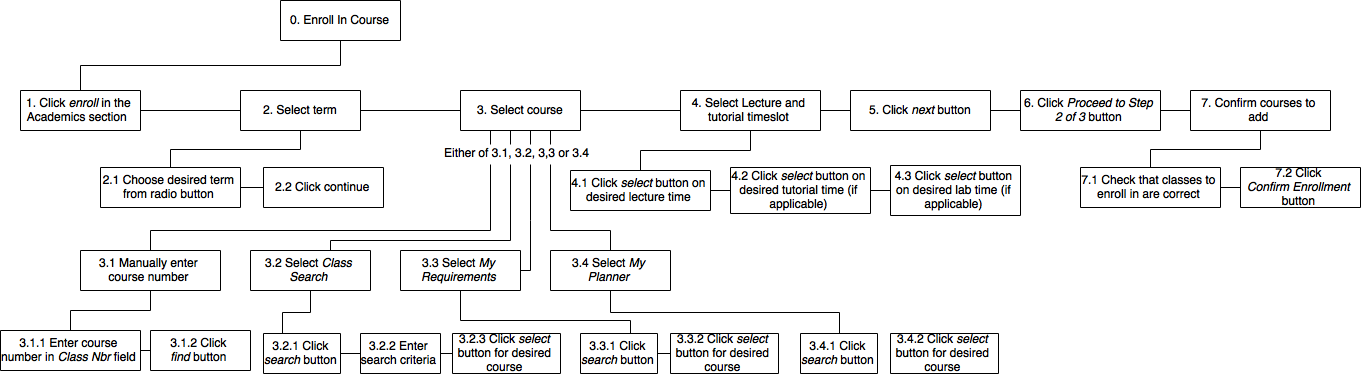
\includegraphics[width=\textwidth]{images/MosaicEnroll.png}}\\
%    \Caption{Mosaic HTA -- Enrolling in a Course}
%\end{figure}
%
%\begin{figure}[h]
%    \centering
%    \fbox{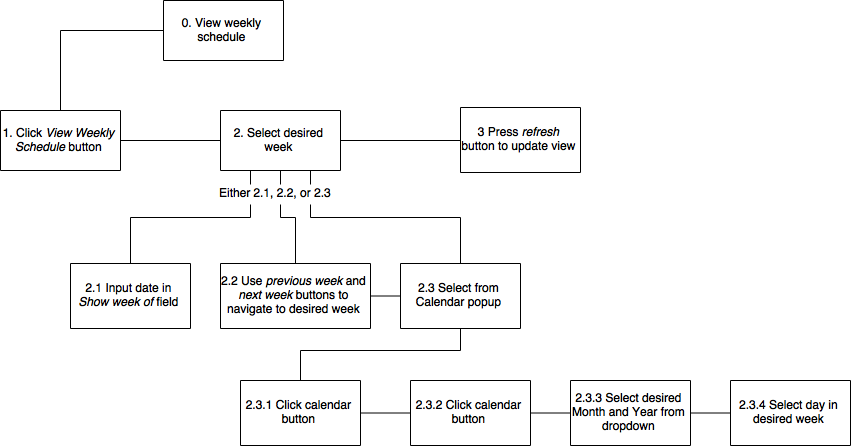
\includegraphics[width=\textwidth]{images/MosaicViewSchedule.png}}\\
%    \Caption{Mosaic HTA -- Viewing Weekly Schedule}
%\end{figure}
%
%\begin{figure}[h]
%    \centering
%    \fbox{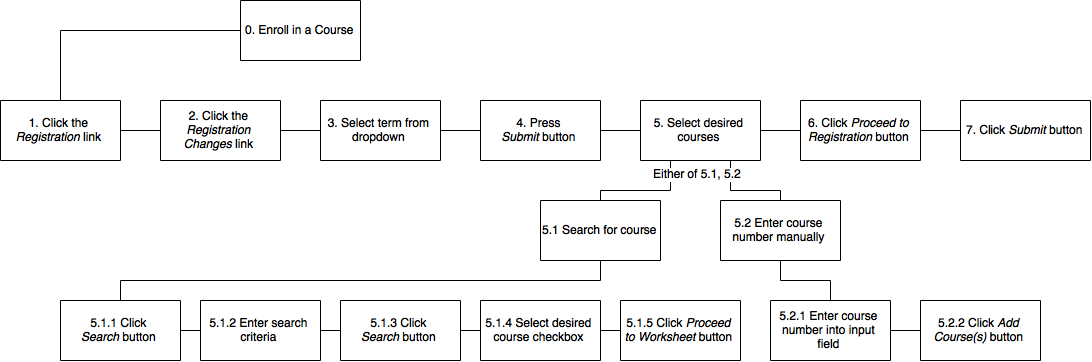
\includegraphics[width=\textwidth]{images/CarletonEnroll.png}}\\
%    \Caption{Carleton HTA -- Enrolling in a Course}
%\end{figure}
%
%\begin{figure}[h]
%    \centering
%    \fbox{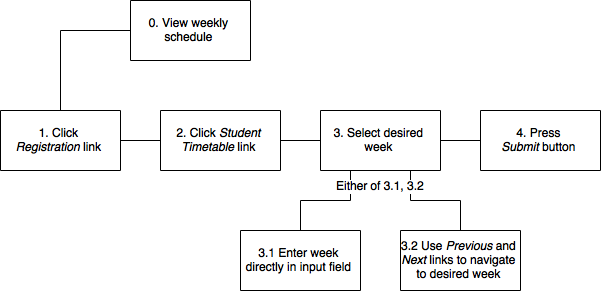
\includegraphics[width=0.6\textwidth]{images/CarletonViewSchedule.png}}\\
%    \Caption{Carleton HTA -- Viewing Weekly Schedule}
%\end{figure}
%
%\begin{figure}[h]
%    \centering
%    \fbox{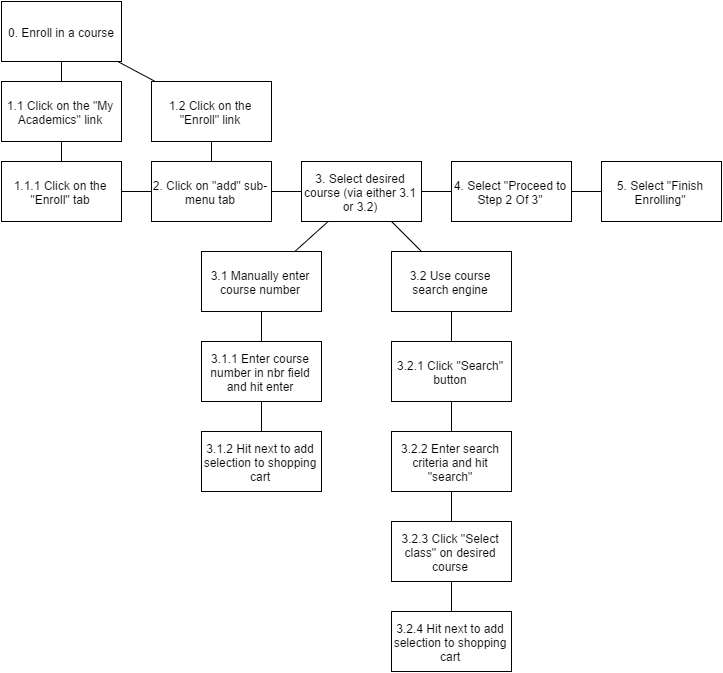
\includegraphics[width=0.6\textwidth]{images/WaterlooEnroll.png}}\\
%    \Caption{Quest HTA -- Enrolling in a Course}
%\end{figure}
%
%\begin{figure}[h]
%    \centering
%    \fbox{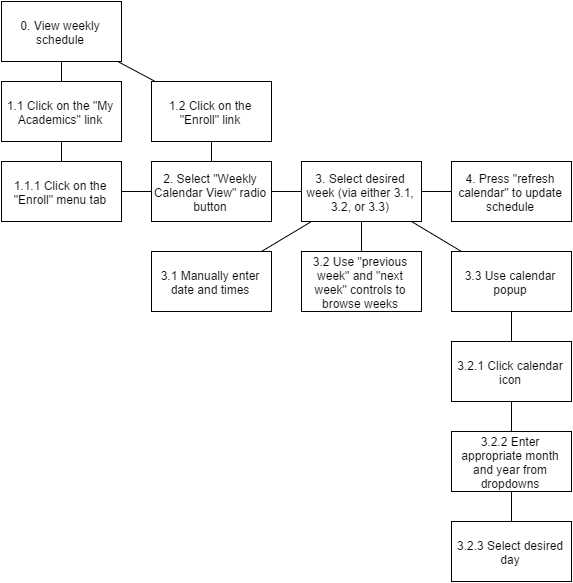
\includegraphics[width=0.6\textwidth]{images/WaterlooSchedule.png}}\\
%    \Caption{Quest HTA -- Viewing Weekly Schedule}
%\end{figure}
%
%\begin{figure}[h]
%    \centering
%    \fbox{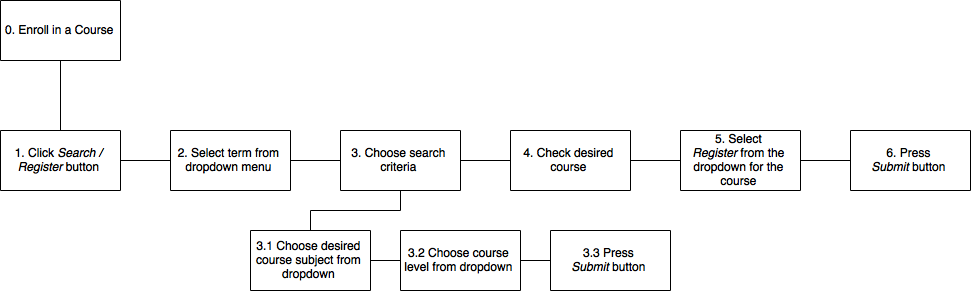
\includegraphics[width=\textwidth]{images/WebAdvisorEnroll.png}}\\
%    \Caption{WebAdvisor HTA -- Enrolling in a Course}
%\end{figure}
%
%\begin{figure}[h]
%    \centering
%    \fbox{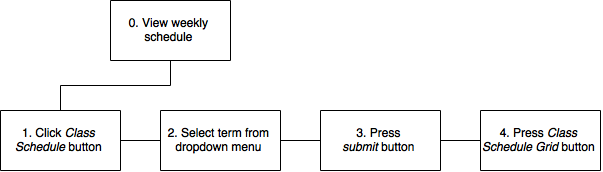
\includegraphics[width=\textwidth]{images/WebAdvisorViewSchedule.png}}\\
%    \Caption{WebAdvisor HTA -- Viewing Weekly Schedule}
%\end{figure}
%
%% ================== SUBSECTION ============================ %
%\clearpage
%\subsection*{Other Systems -- Screenshots}
%
%\begin{minipage}{.5\textwidth}
%    \centering
%    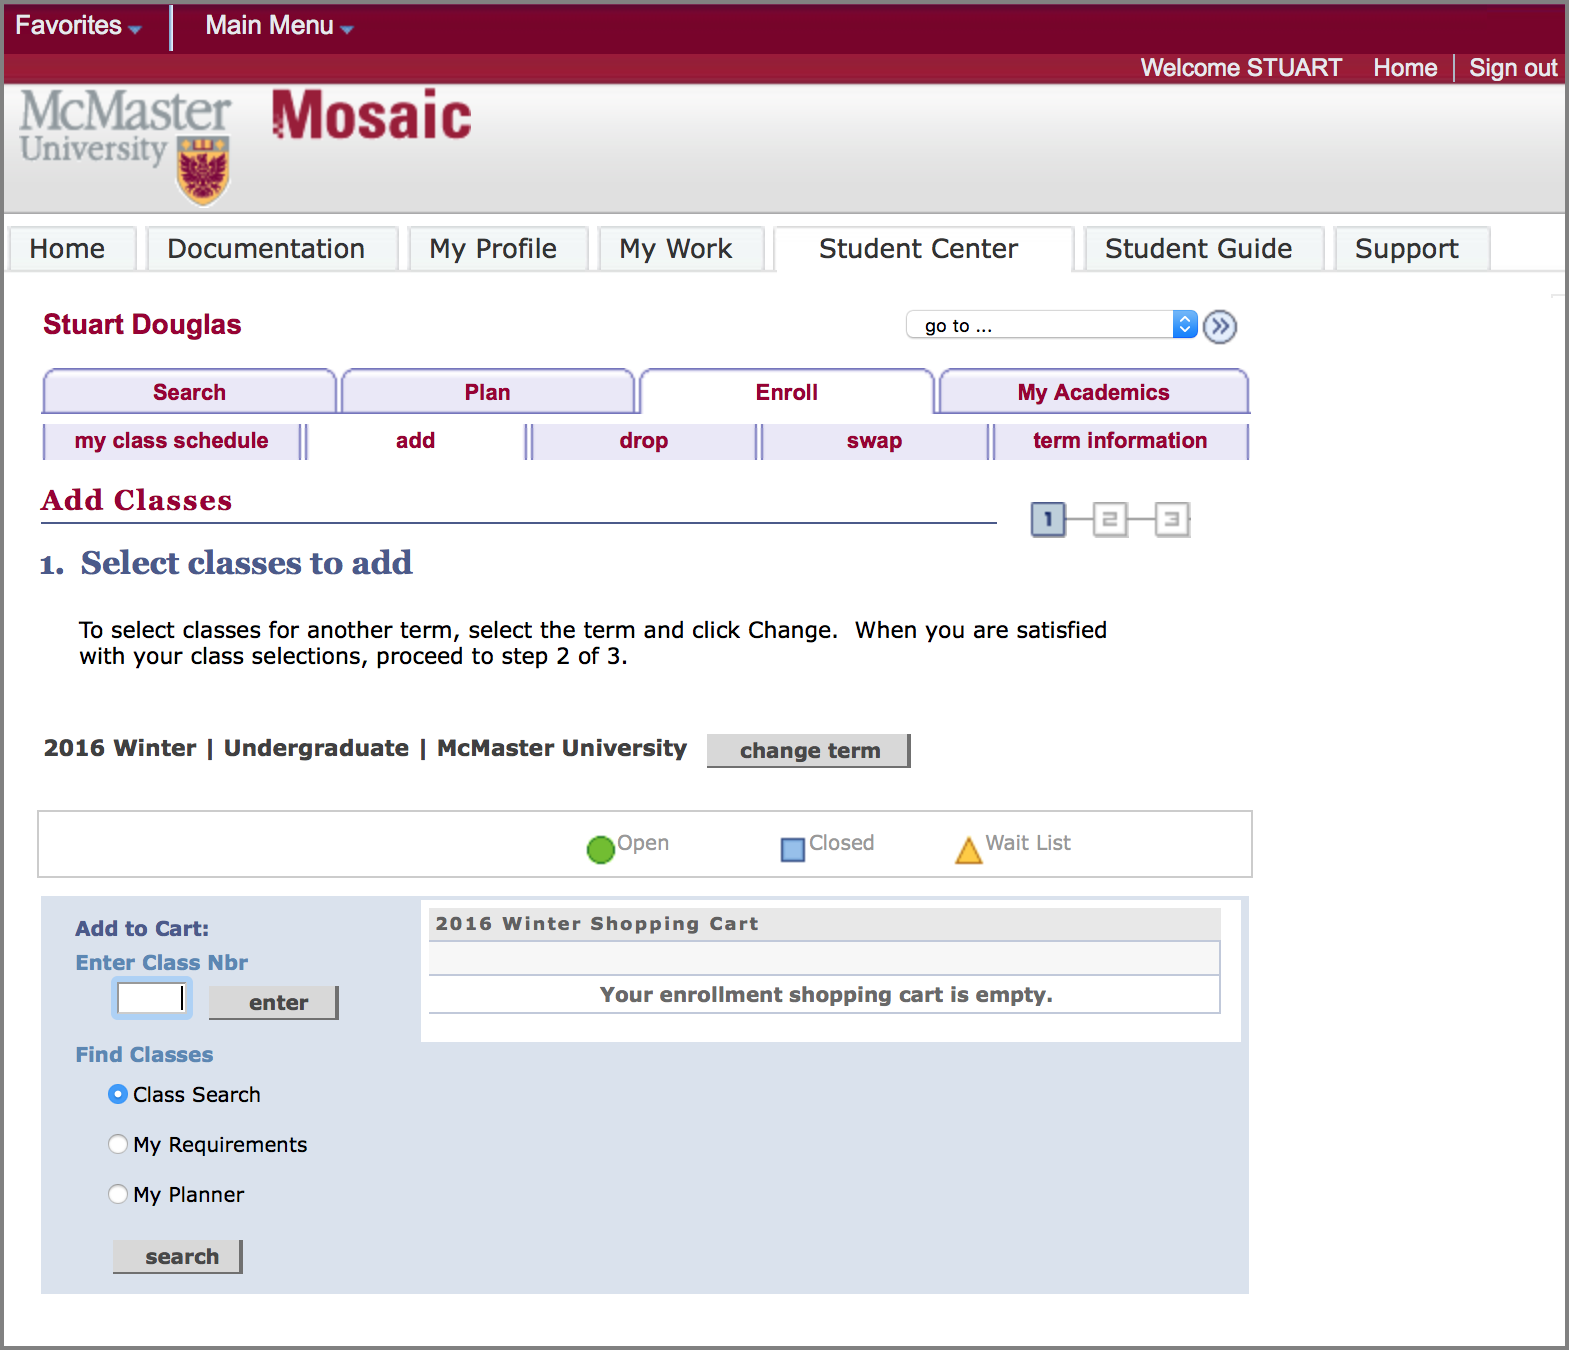
\includegraphics[height=70mm]{images/MosaicScreen.png}\\
%    \Caption{Mosaic -- Screenshot}
%\end{minipage}
%\begin{minipage}{.5\textwidth}
%    \centering
%    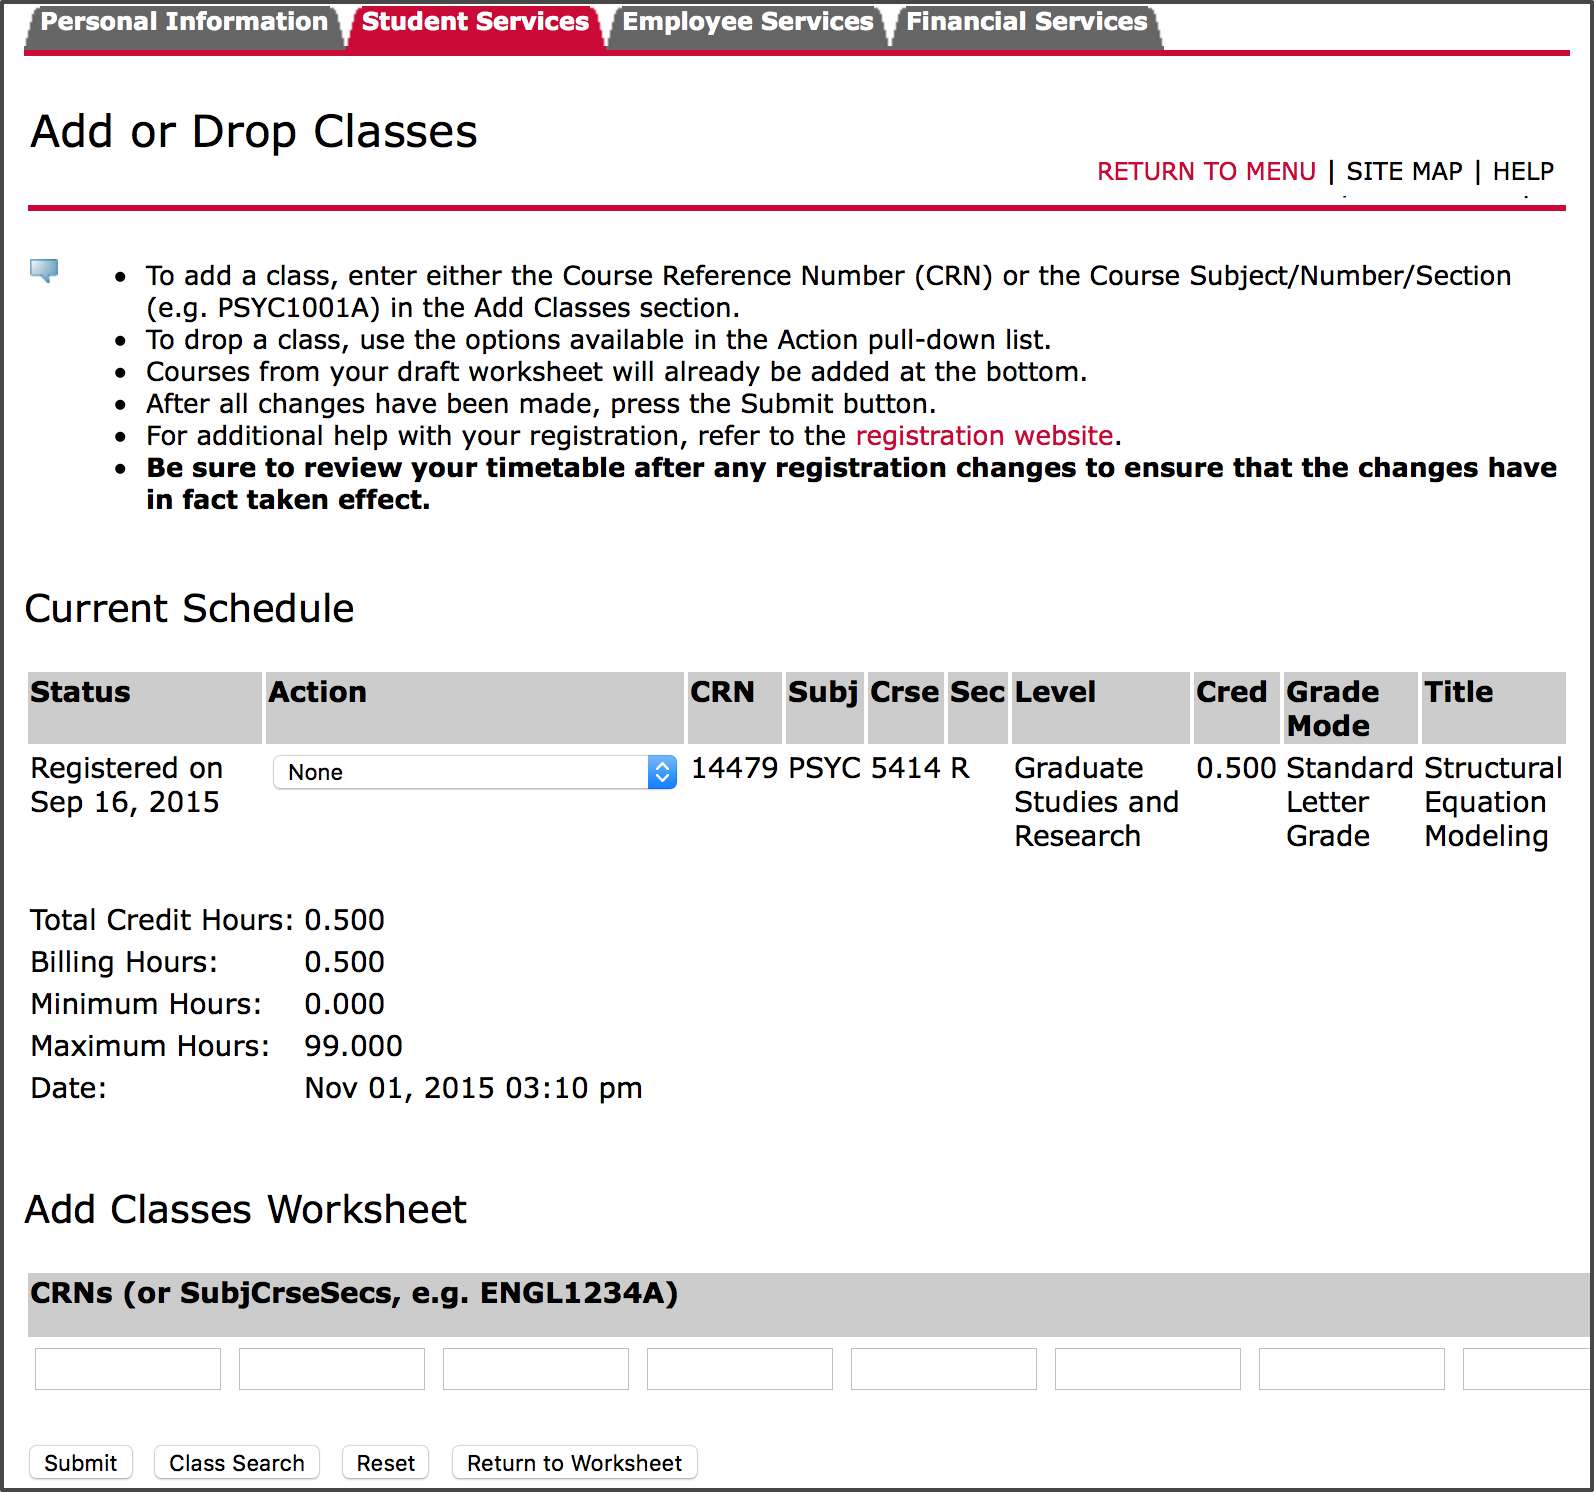
\includegraphics[height=70mm]{images/CarletonScreen.png}\\
%    \Caption{Carleton -- Screenshot}
%\end{minipage}\\\vspace{5mm}
%
%\begin{minipage}{.5\textwidth}
%    \centering
%    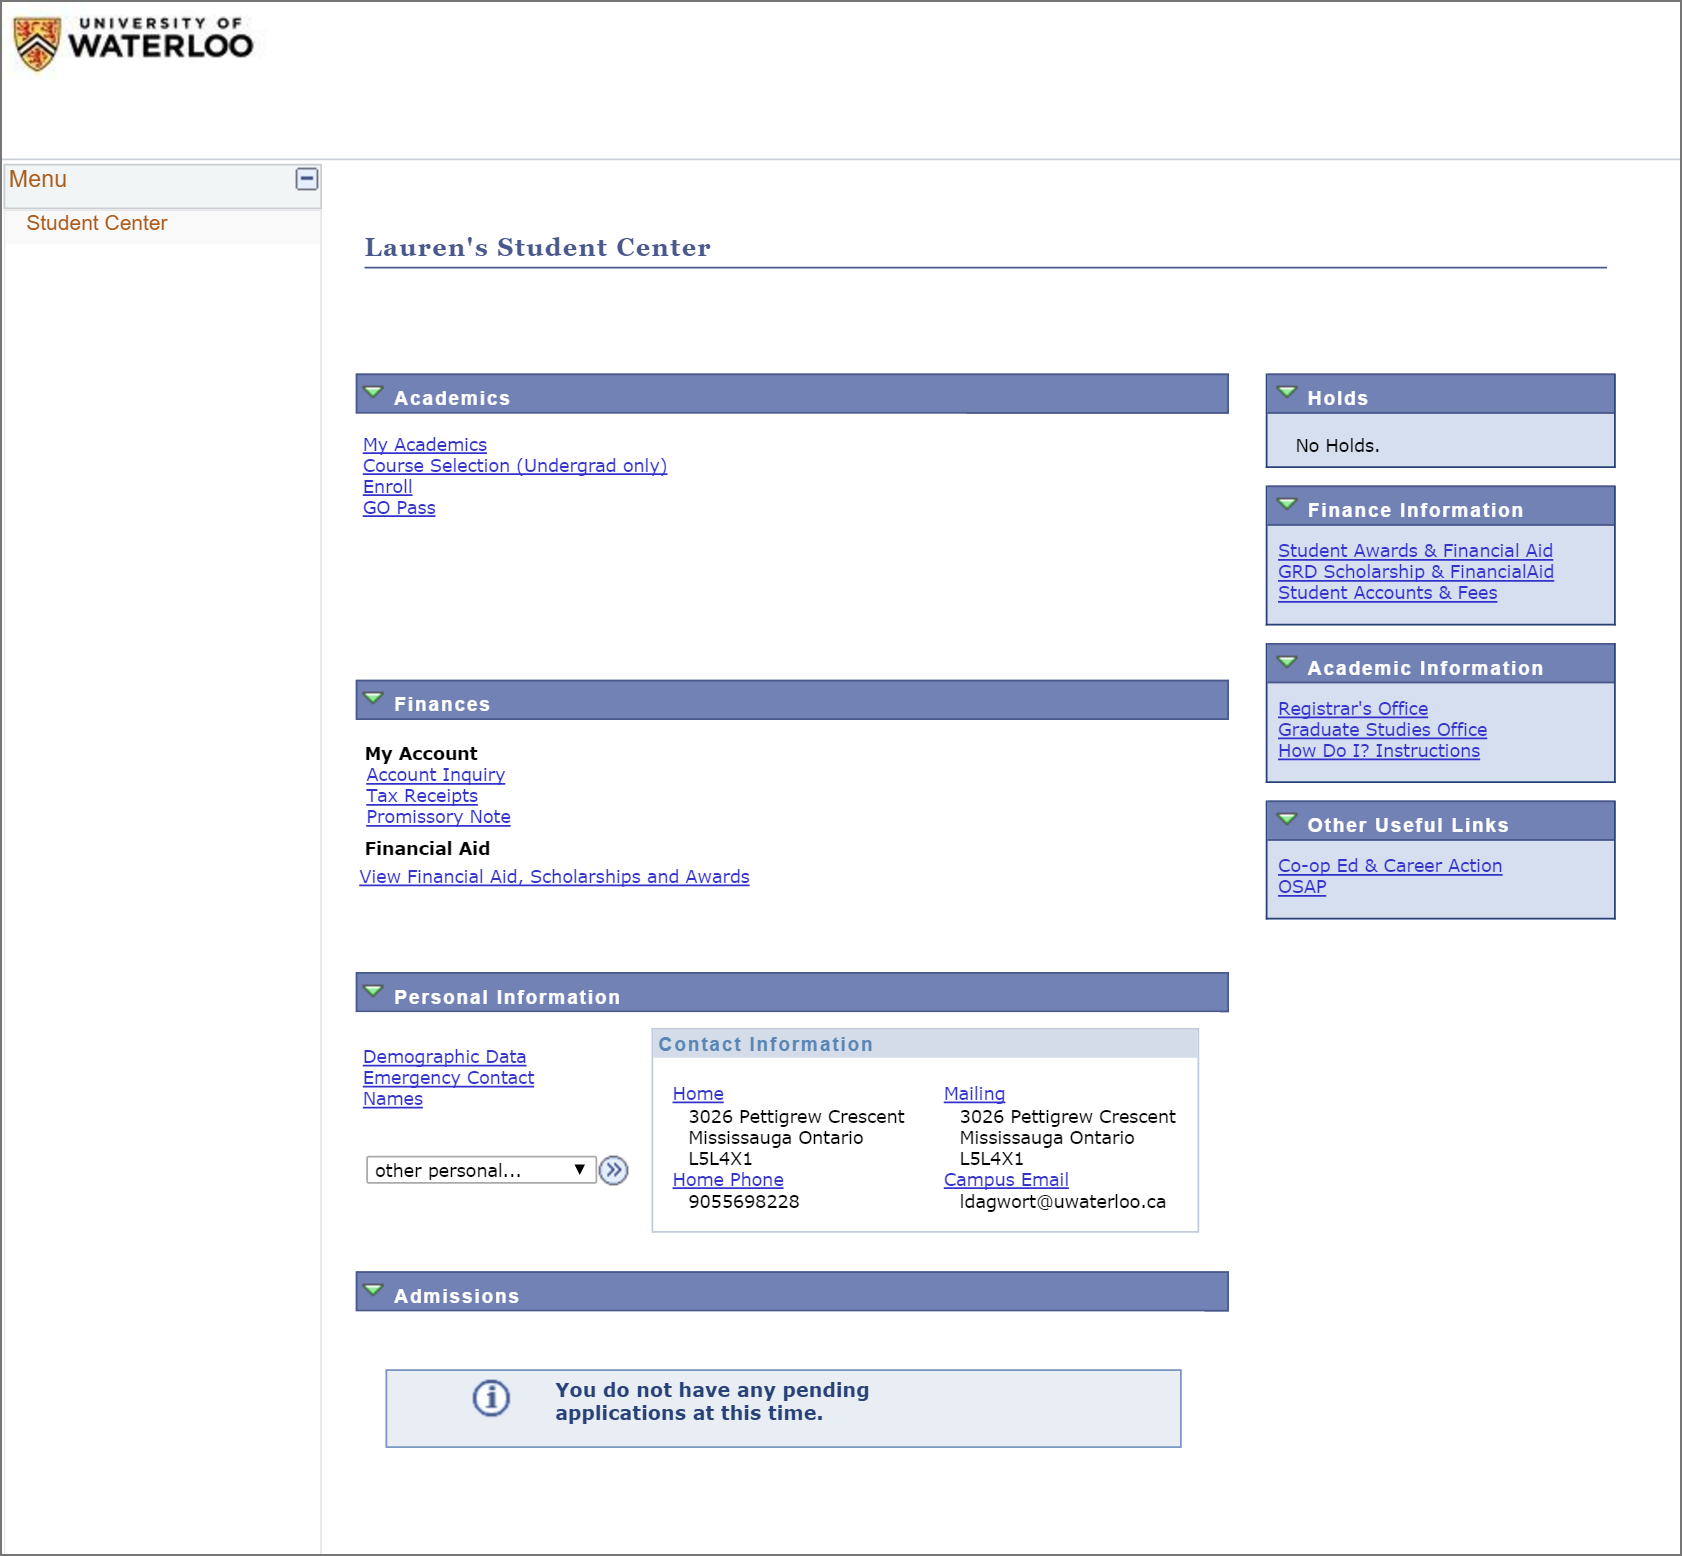
\includegraphics[height=70mm]{images/WaterlooScreen.png}\\
%\Caption{Quest -- Screenshot}
%\end{minipage}
%\begin{minipage}{.5\textwidth}
%    \centering
%	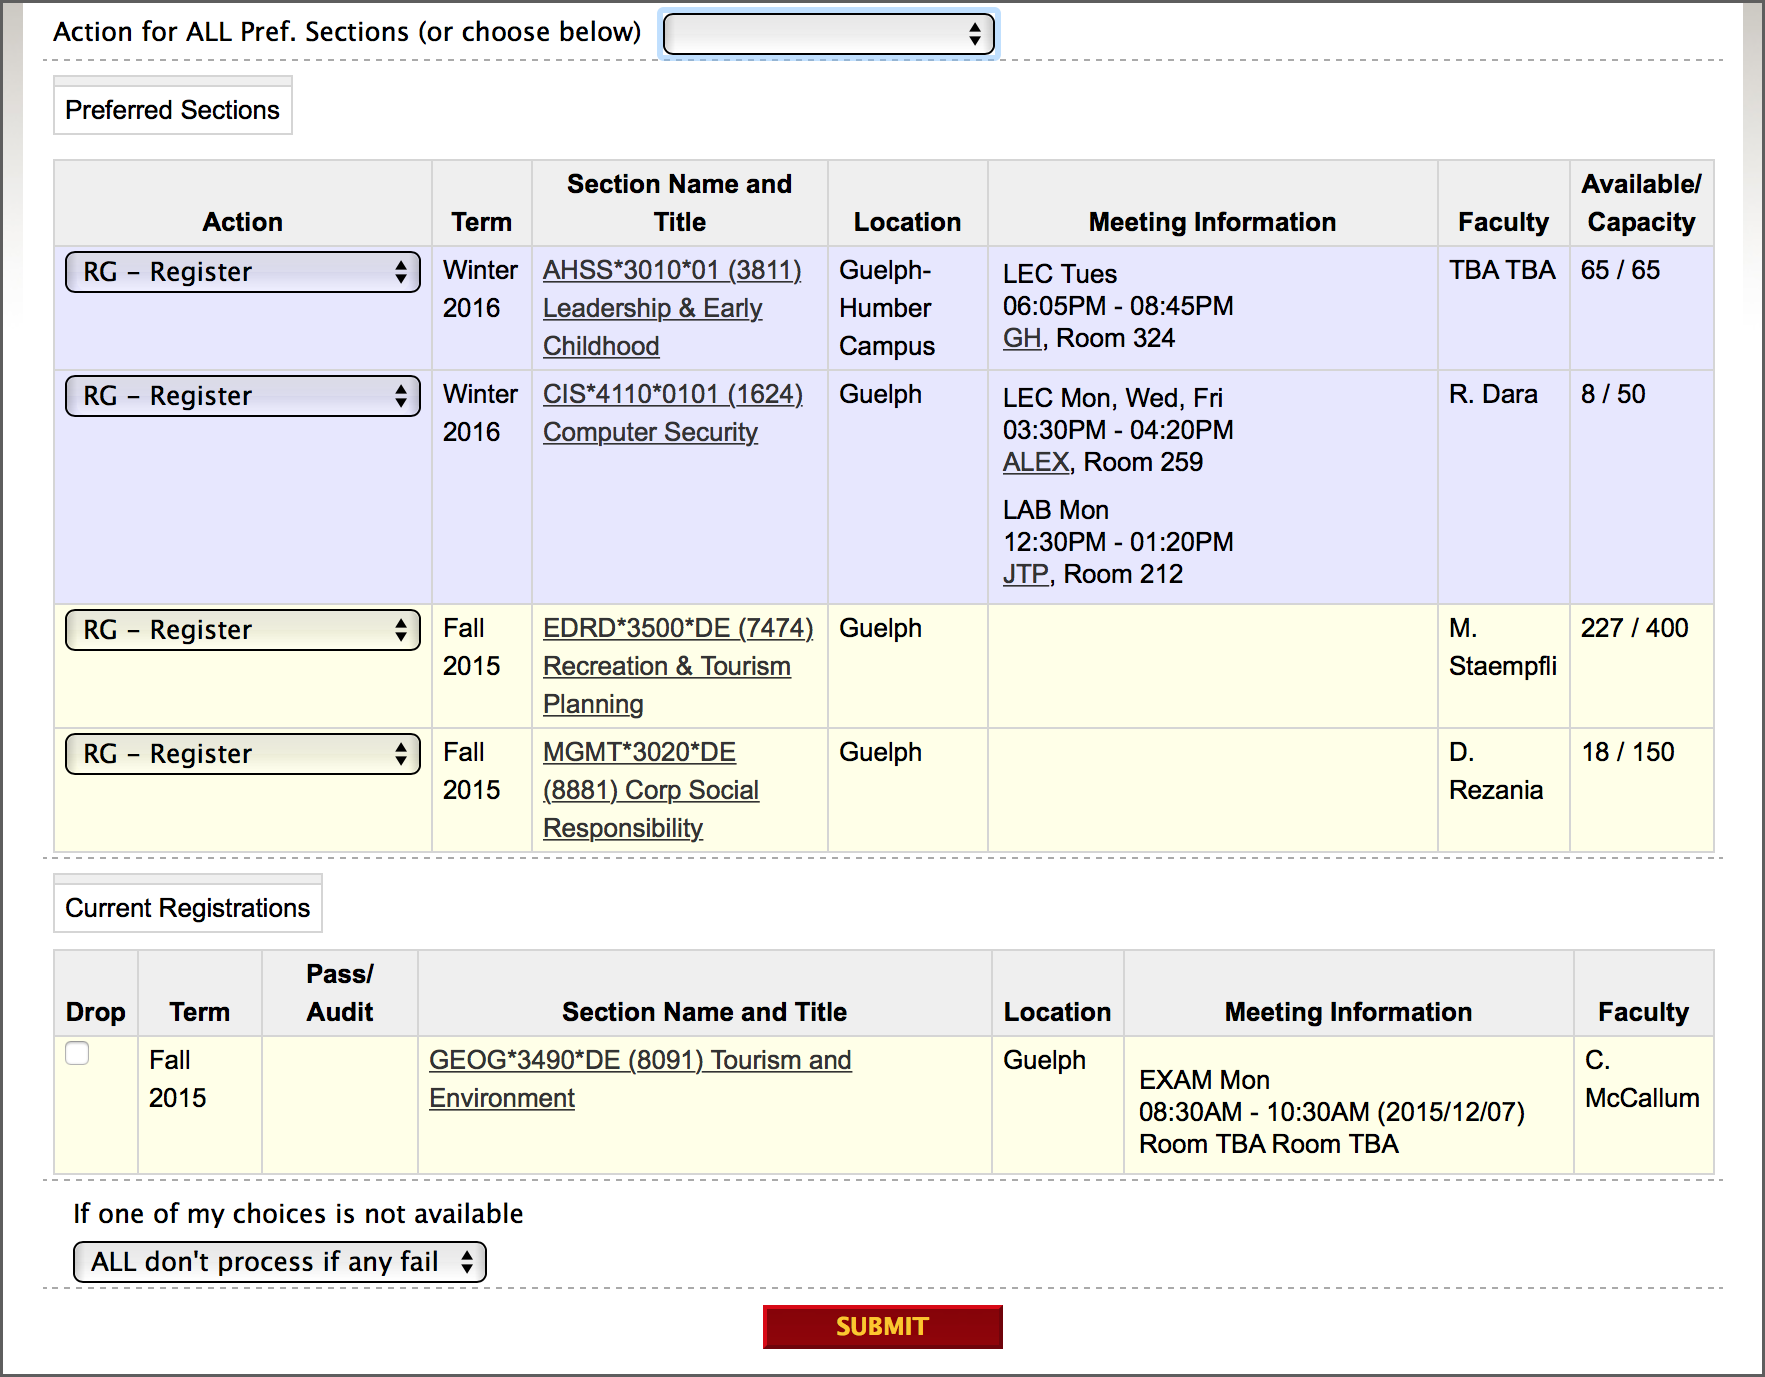
\includegraphics[height=70mm]{images/WebAdvisorScreen.png}\\
%	\Caption{WebAdvisor -- Screenshot}
%\end{minipage}\\\vspace{3mm}
%
%% ================== SUBSECTION ============================ %
%\subsection*{New System -- Final Design Mockups}
%\begin{minipage}{.5\textwidth}
%    \centering
%    \fbox{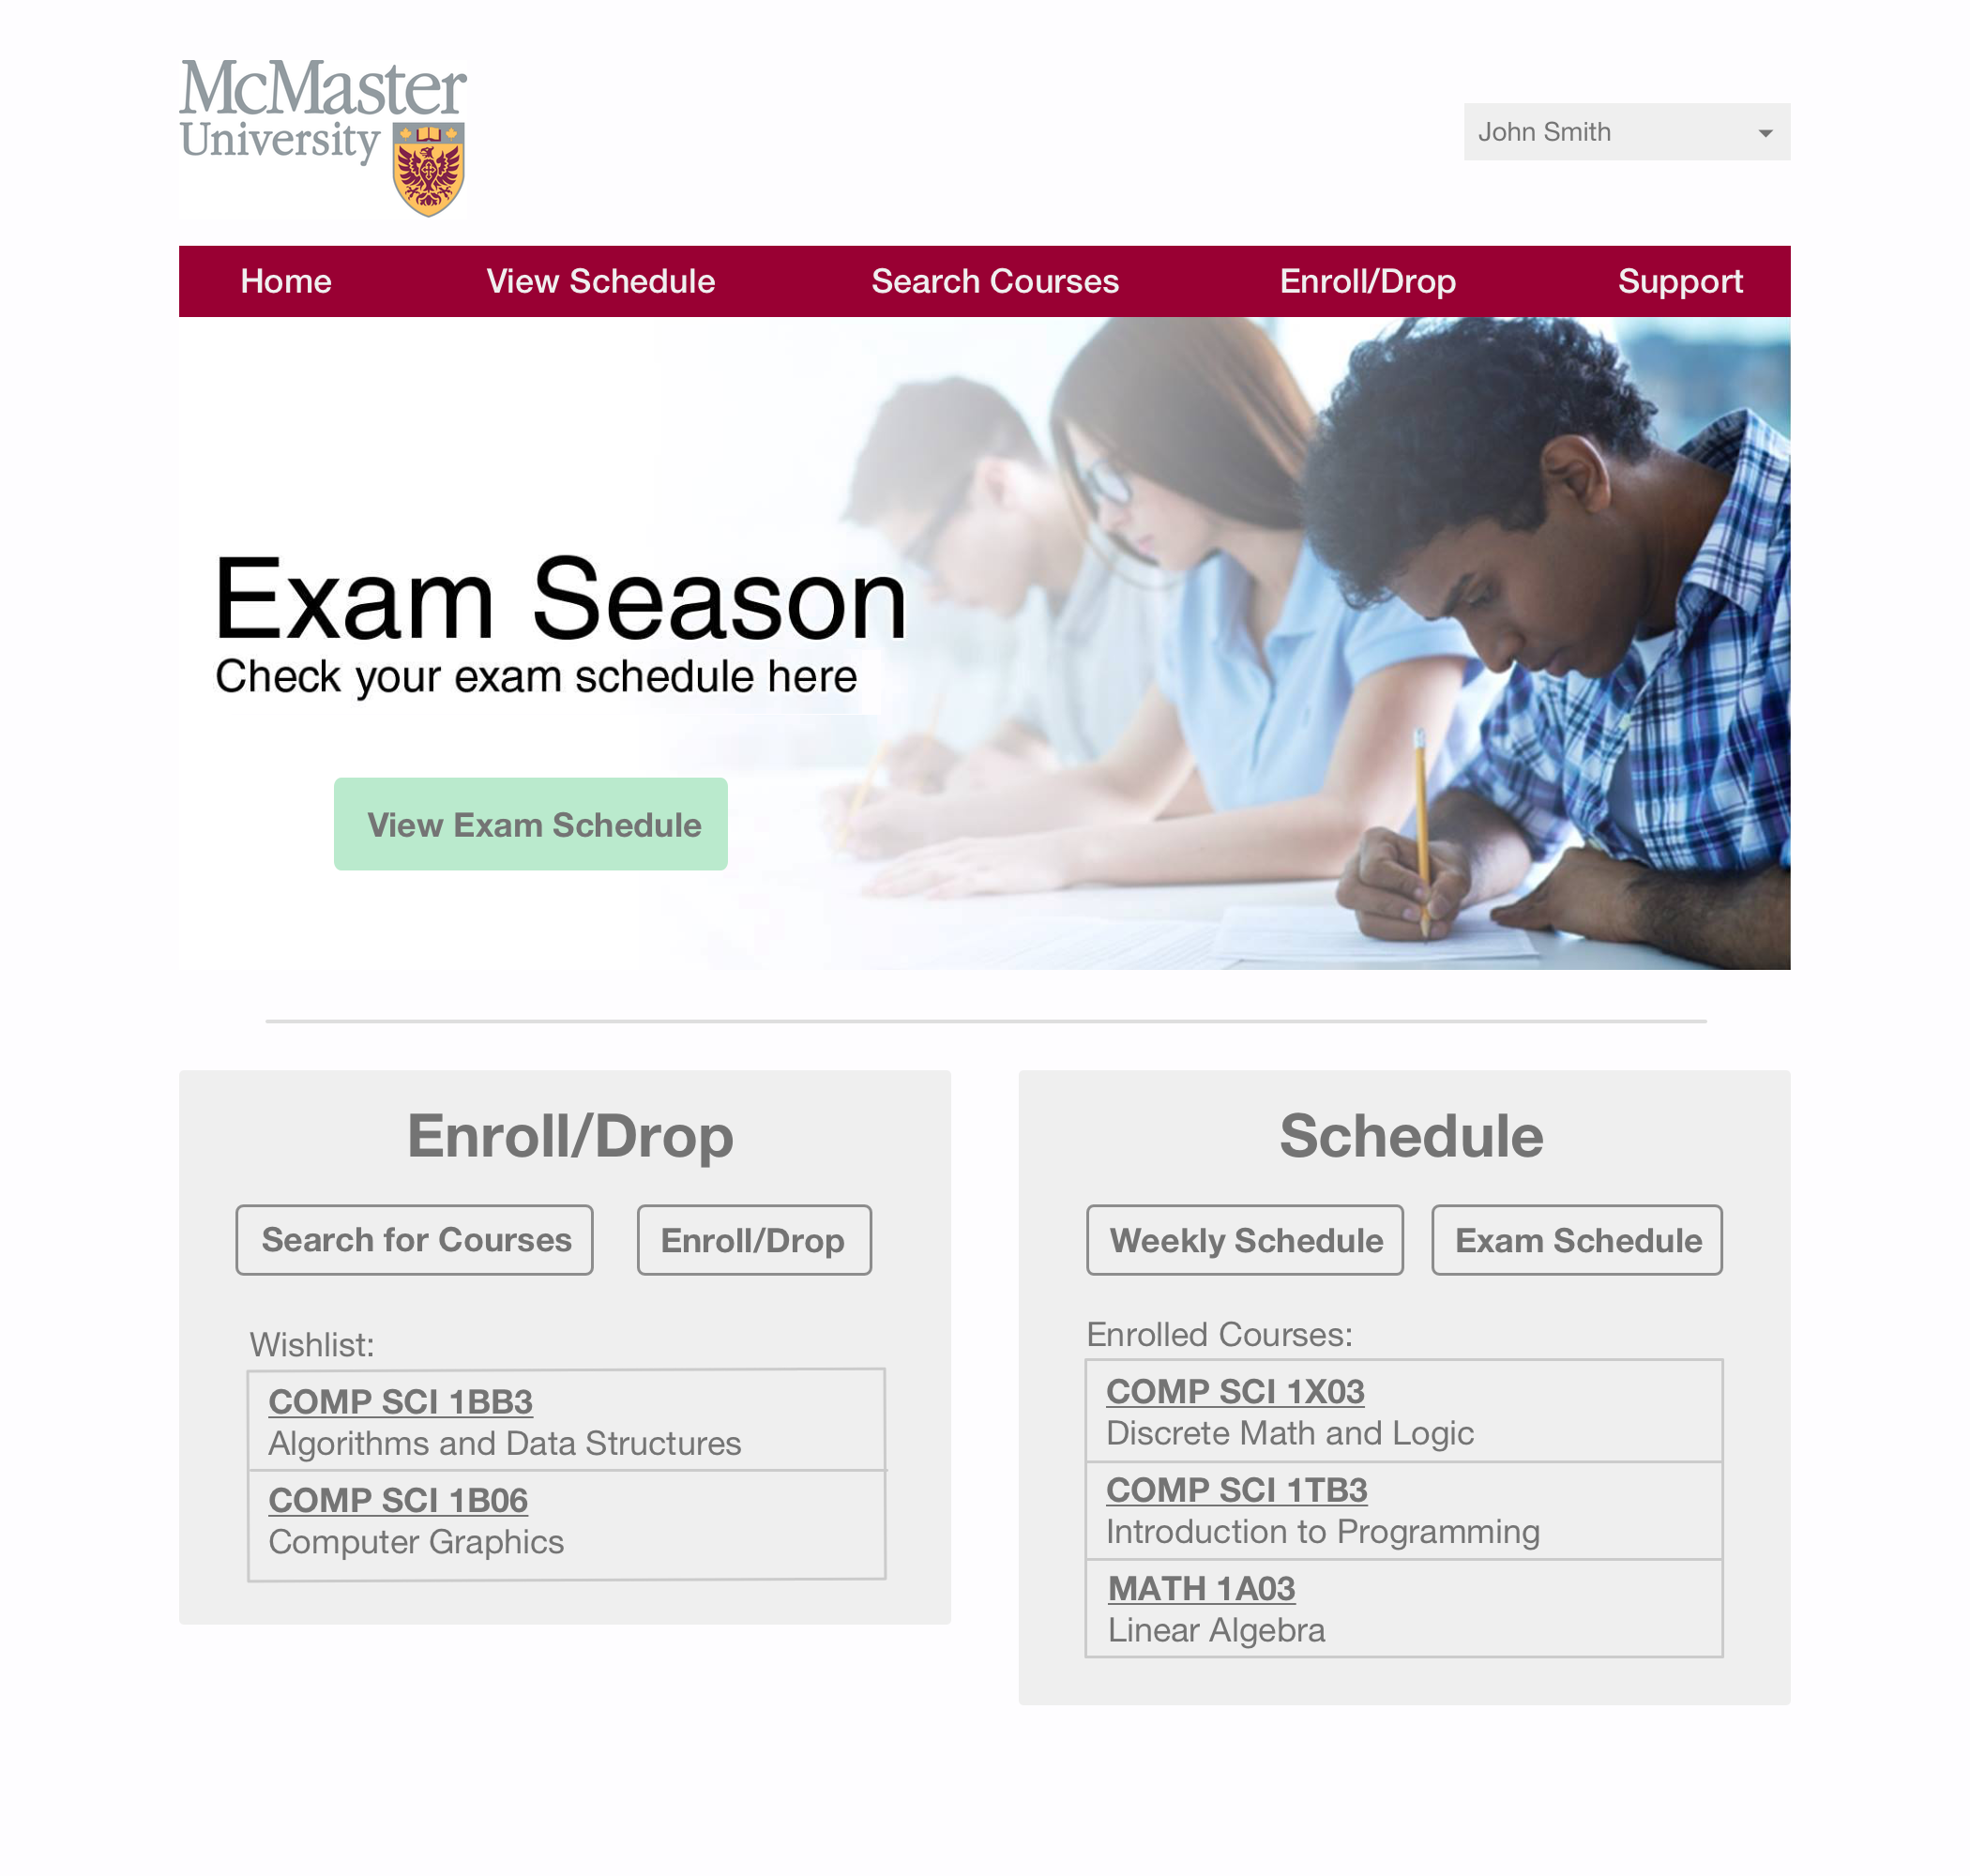
\includegraphics[height=80mm]{images/Rev2_MainPage.png}}\\
%    \Caption{Final Mockup of Home Page}
%\end{minipage}
%\begin{minipage}{.5\textwidth}
%    \centering
%    \fbox{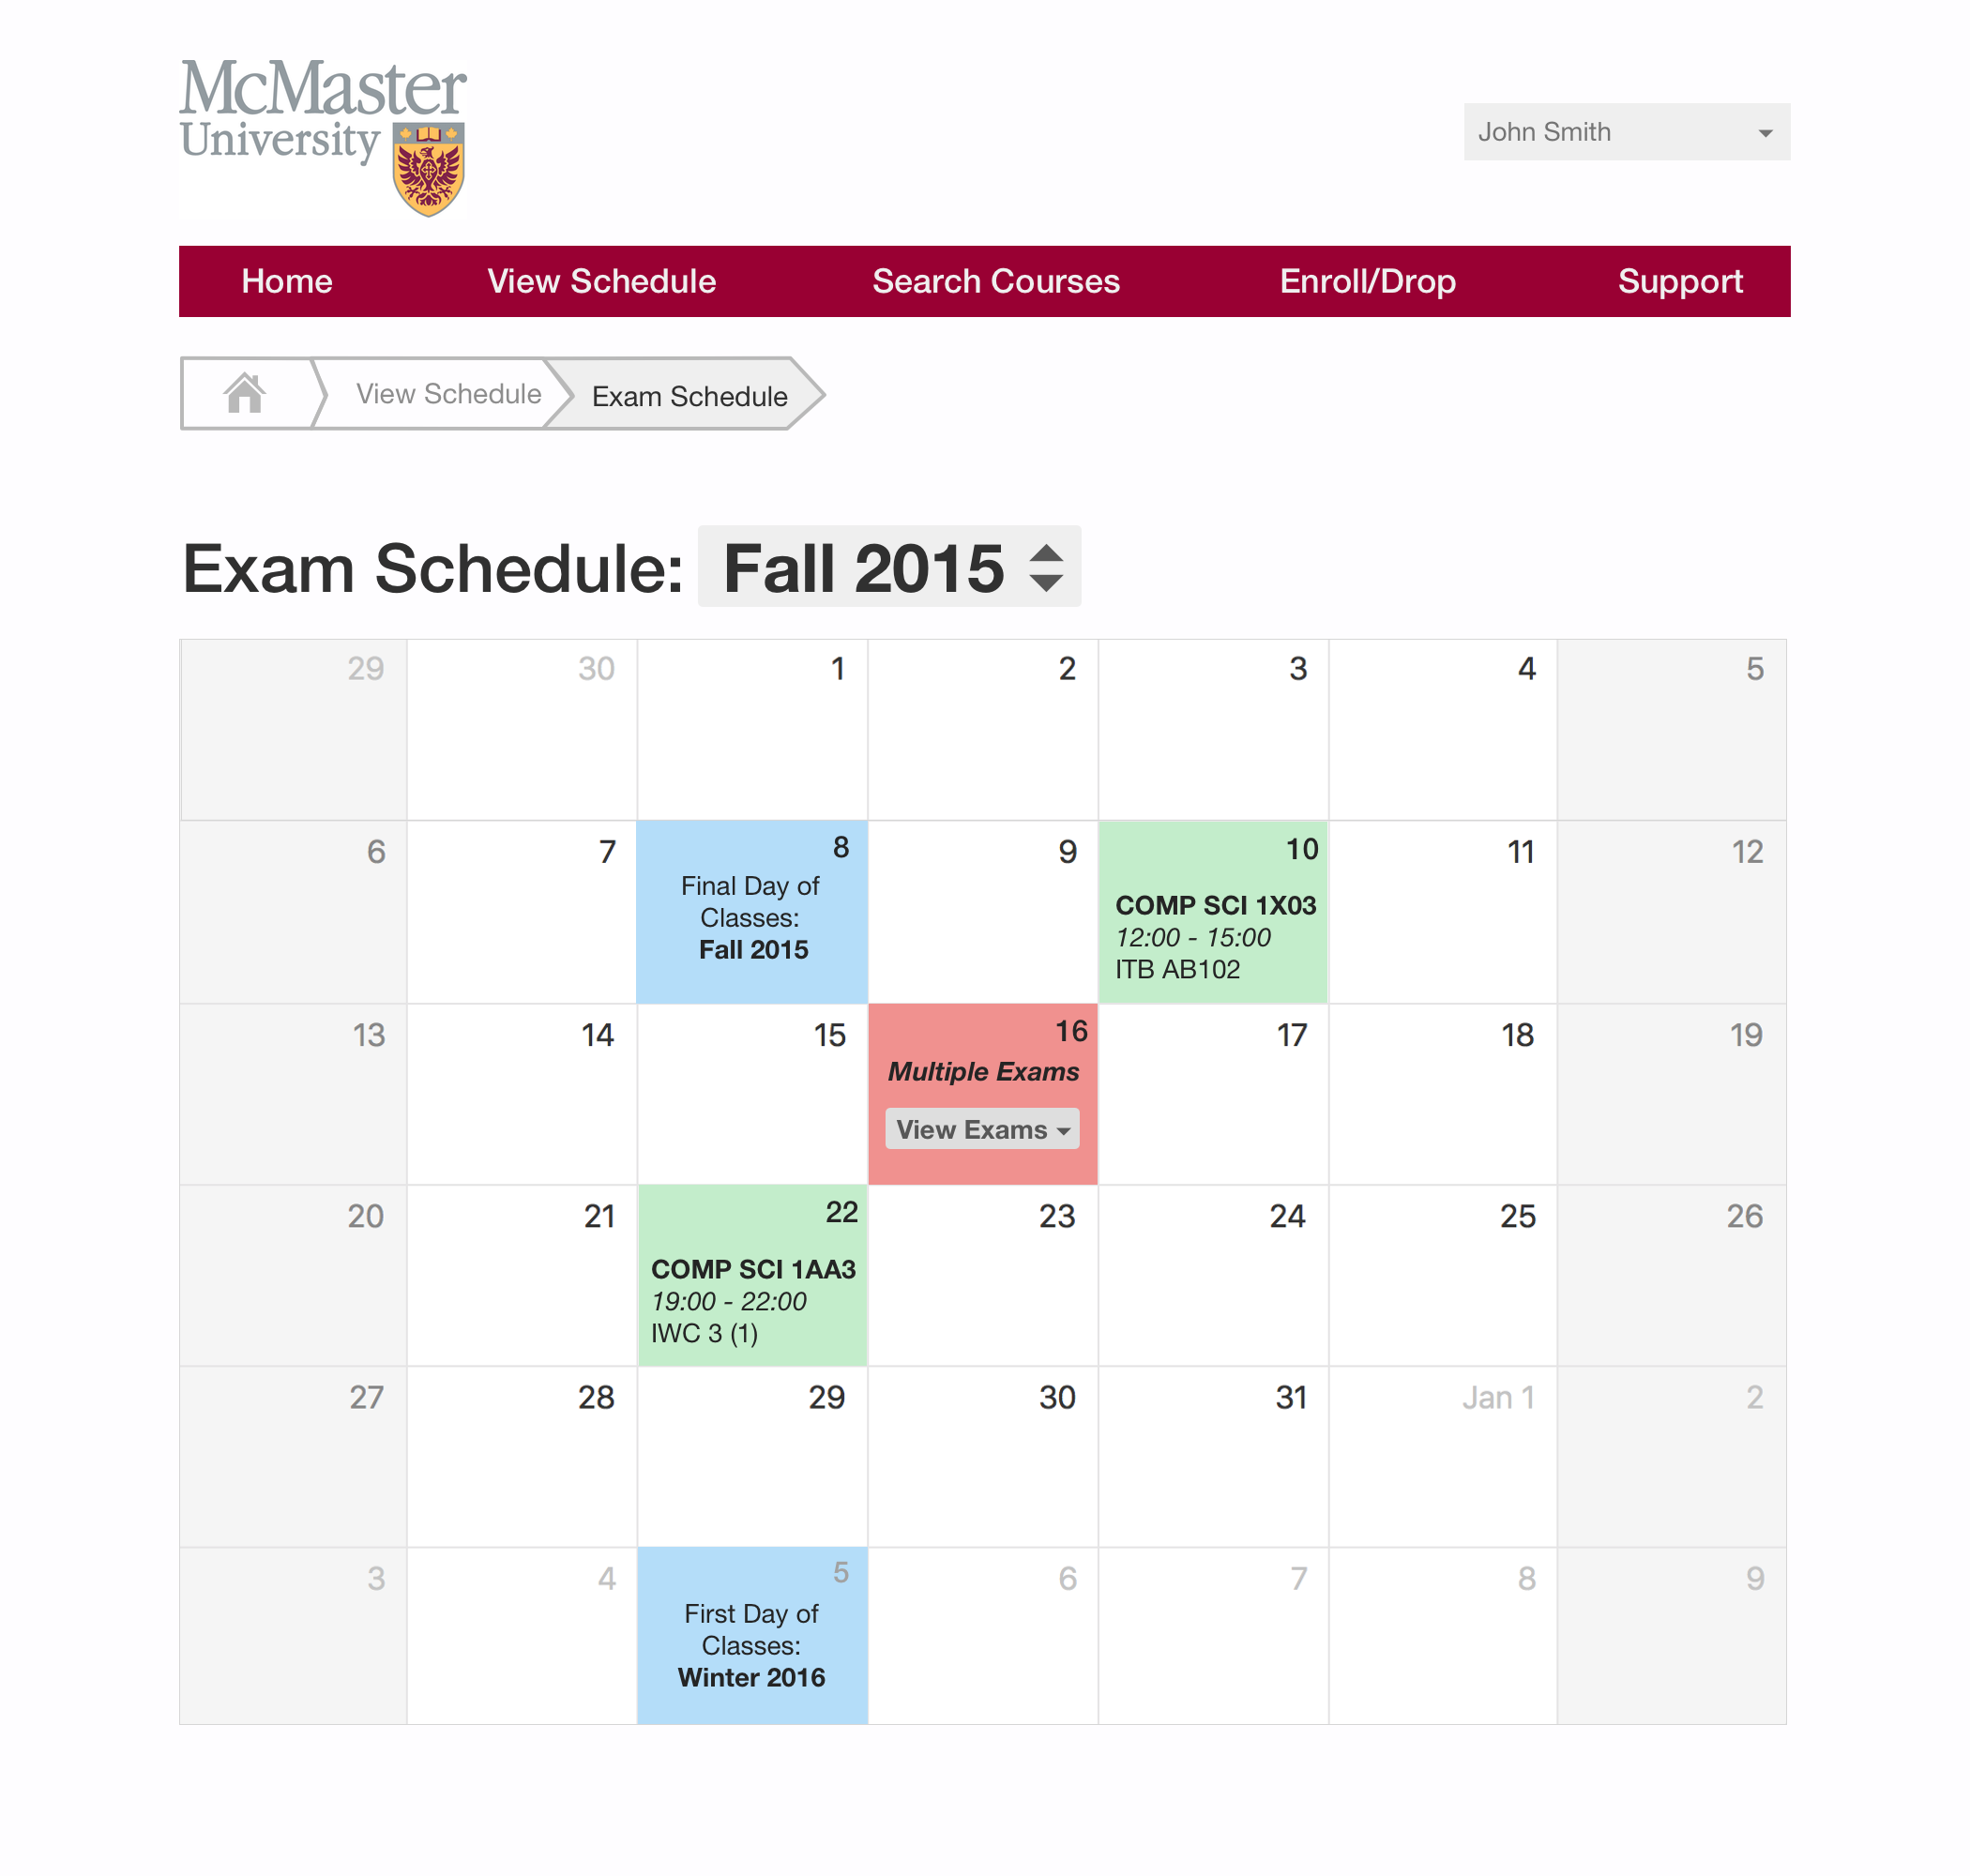
\includegraphics[height=80mm]{images/Rev2_ExamSchedule.png}}\\
%    \Caption{Final Mockup of Exam Schedule}
%\end{minipage}\\\vspace{5mm}
%
%\begin{minipage}{.5\textwidth}
%    \centering
%    \fbox{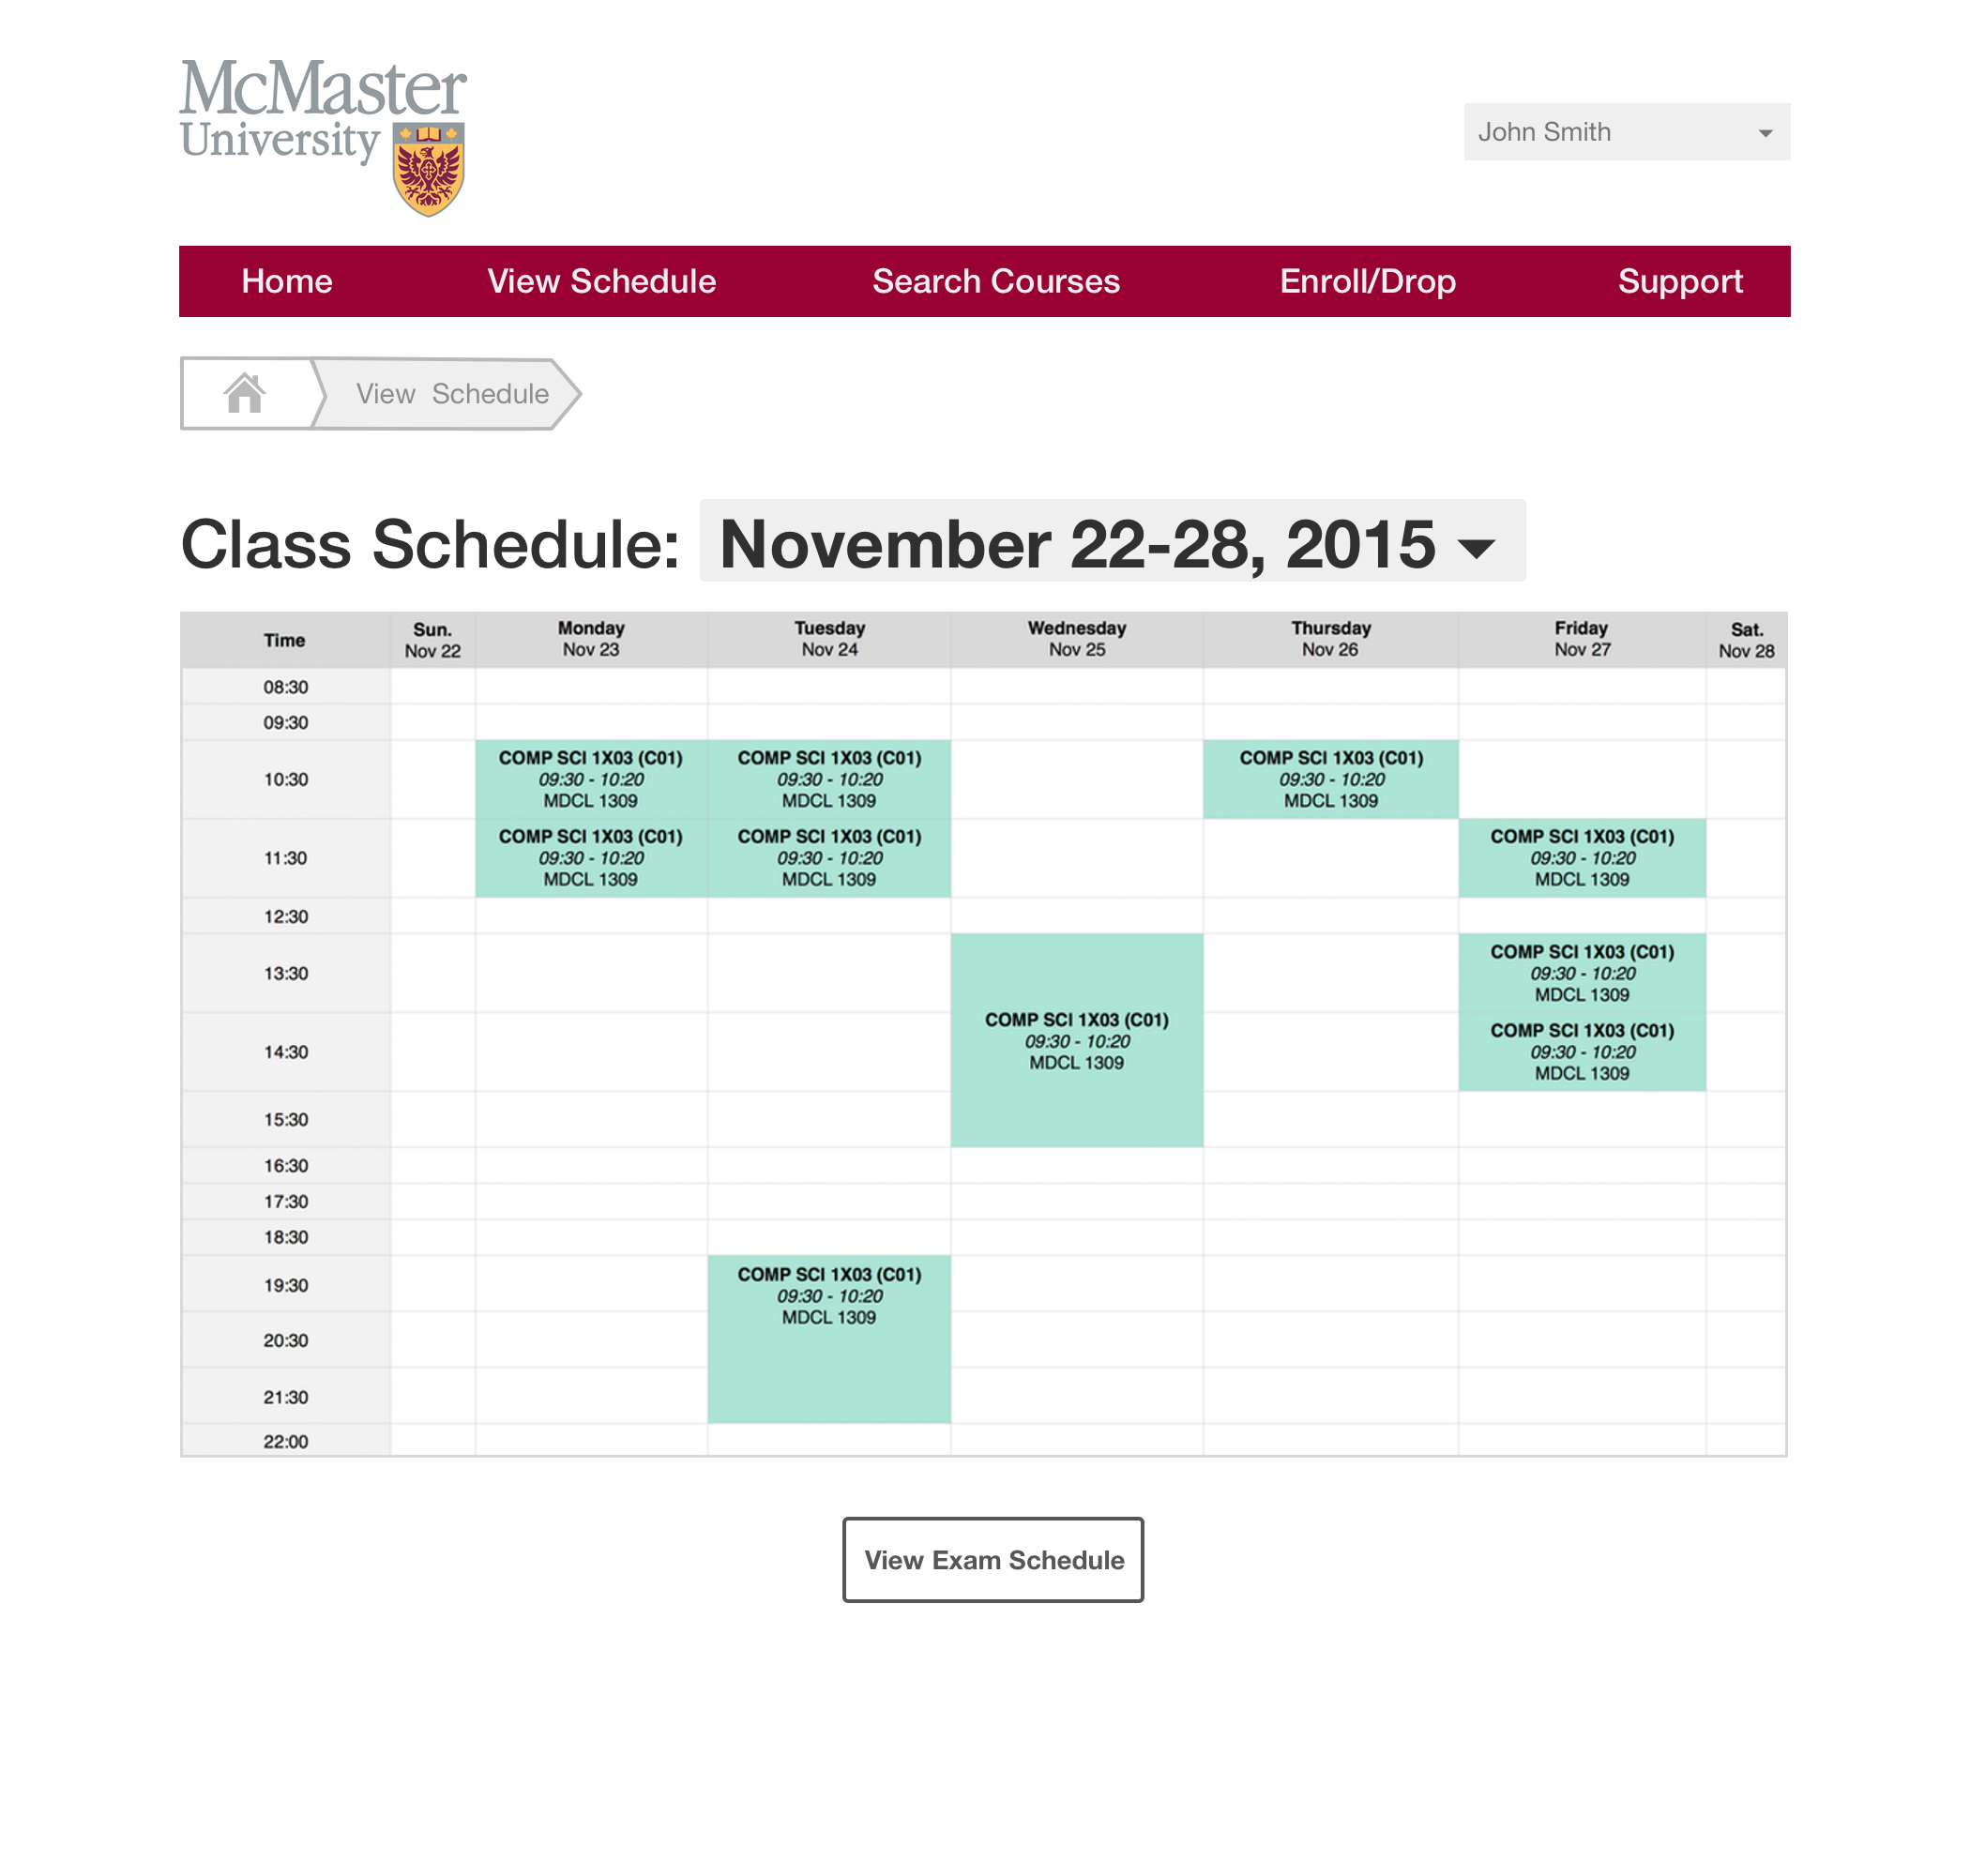
\includegraphics[height=80mm]{images/Rev2_WeeklySchedule.png}}\\
%	\Caption{Final Mockup of Weekly Schedule}
%\end{minipage}
%\begin{minipage}{.5\textwidth}
%    \centering
%	\fbox{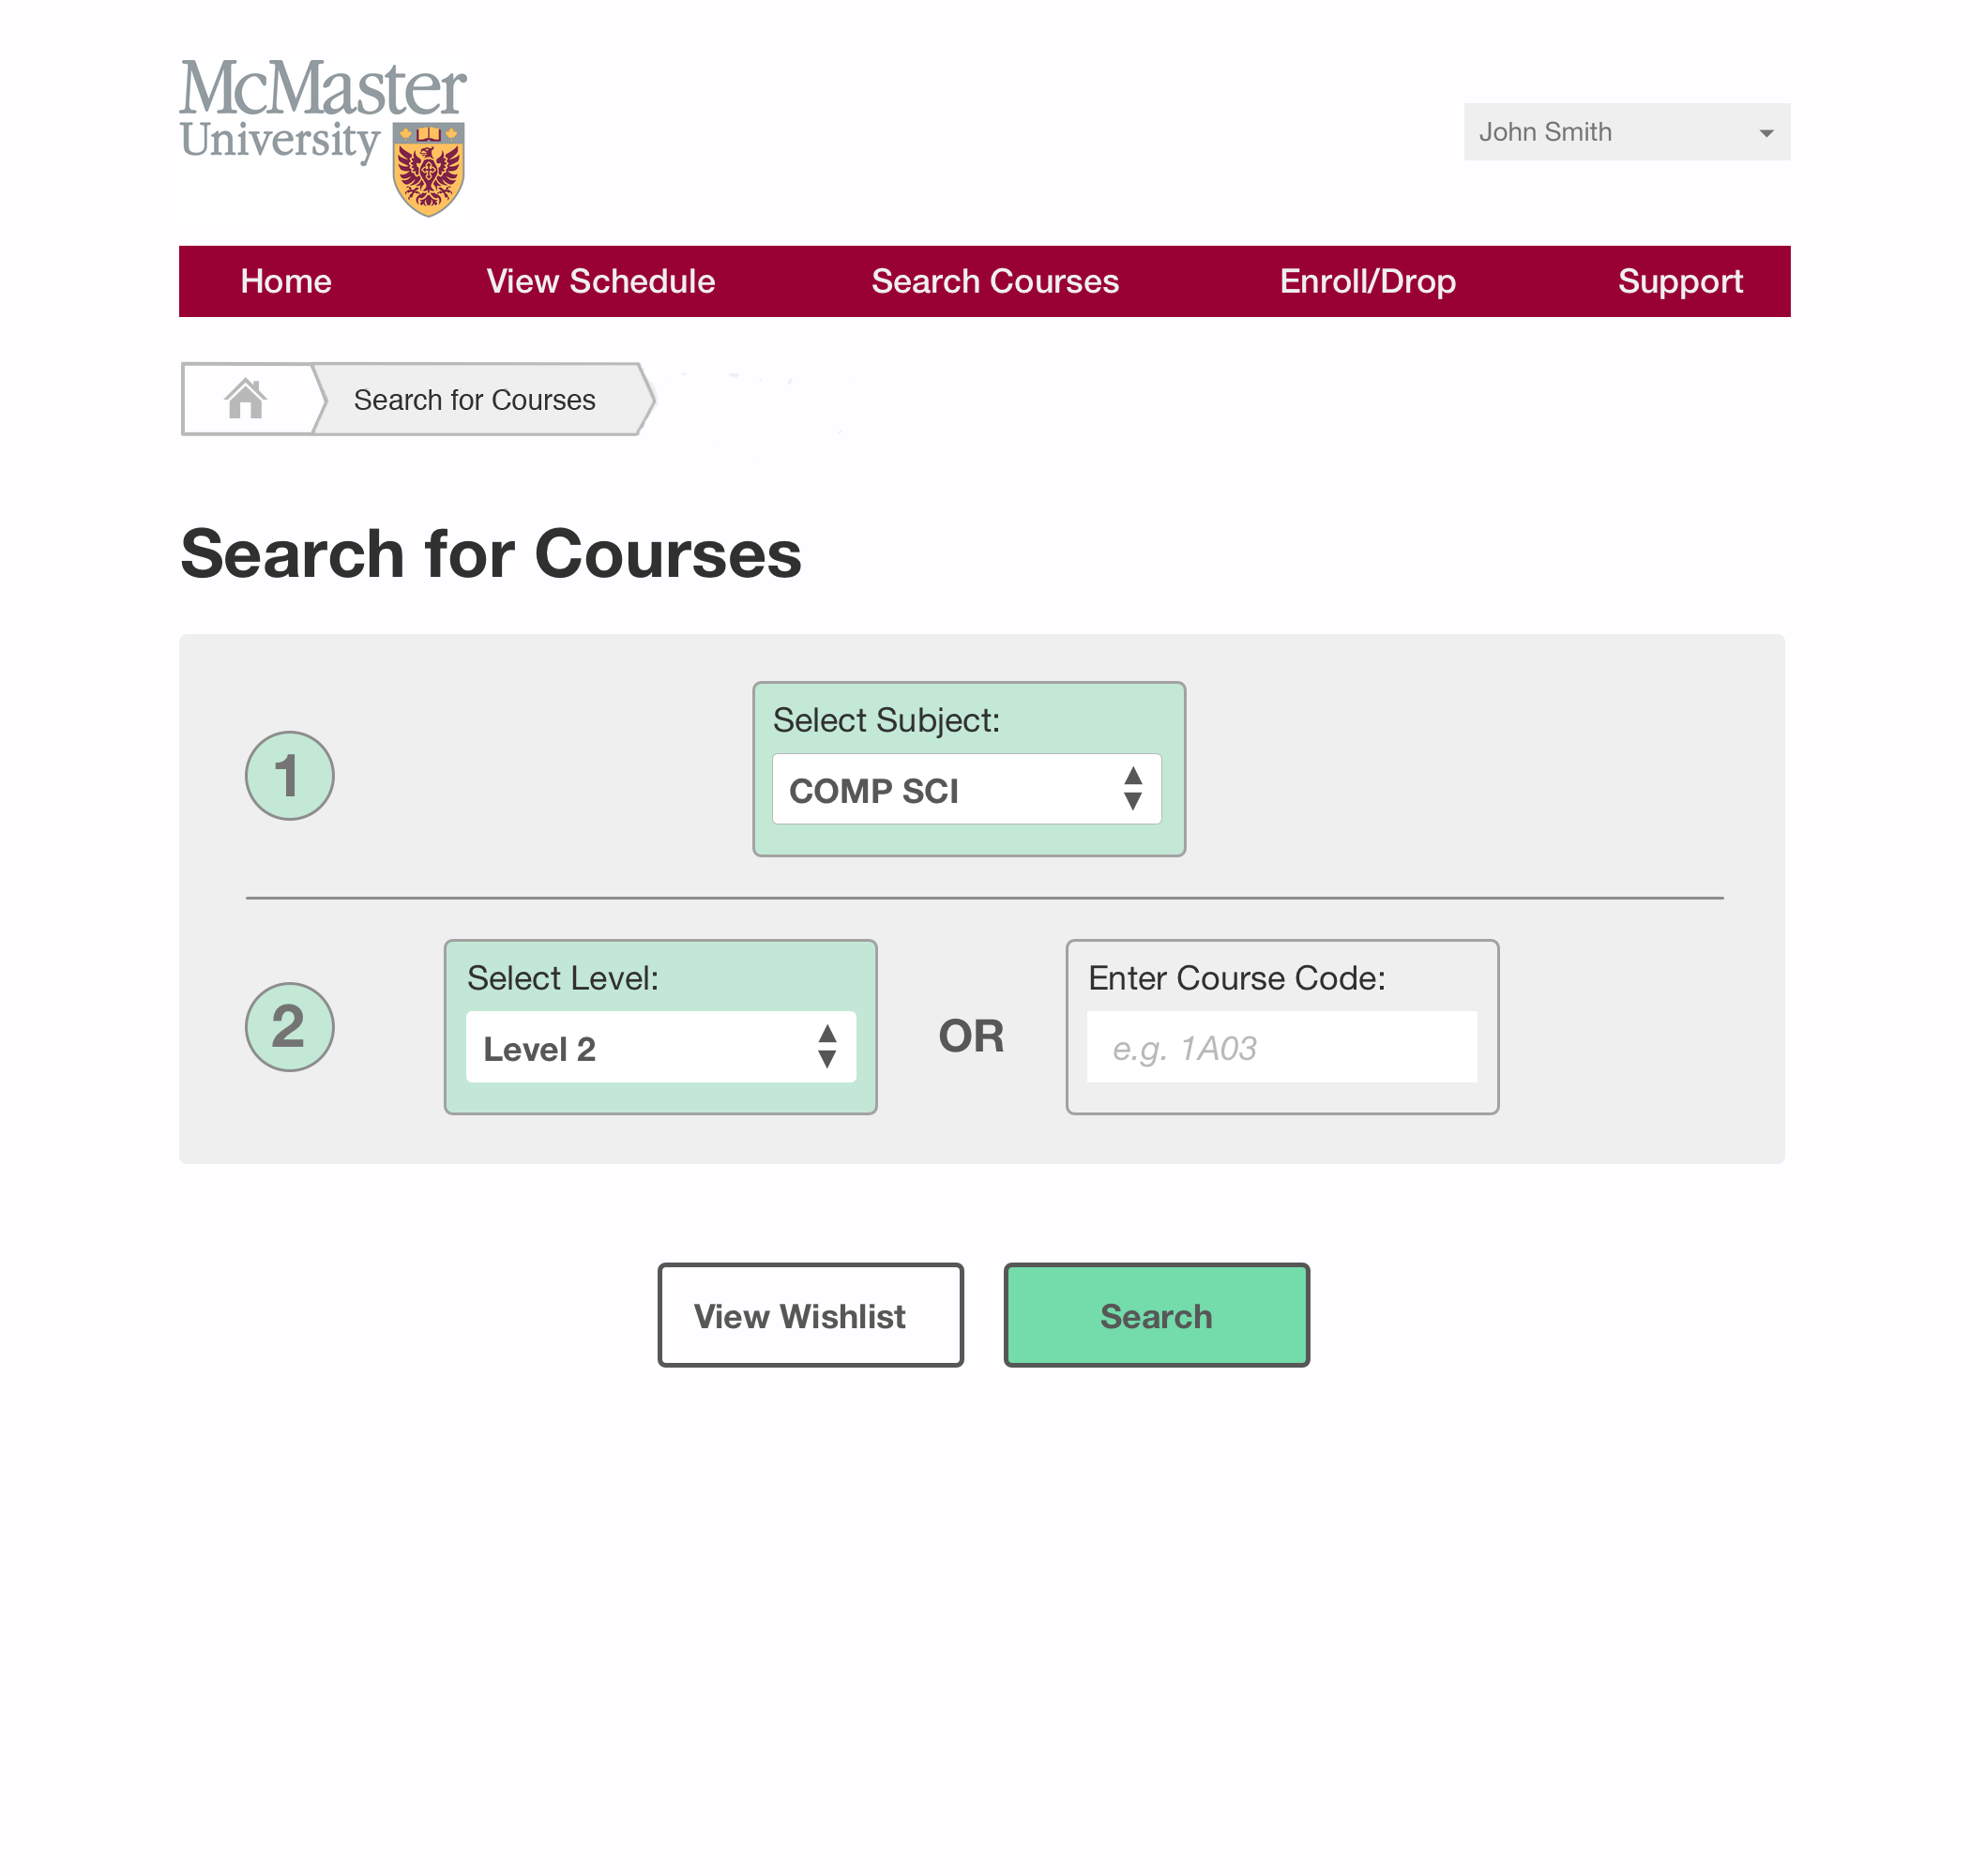
\includegraphics[height=80mm]{images/Rev2_SearchCourses.png}}\\
%	\Caption{Final Mockup of Search Criteria Page}
%\end{minipage}\\\vspace{3mm}
%
%\begin{minipage}{.5\textwidth}
%    \centering
%    \fbox{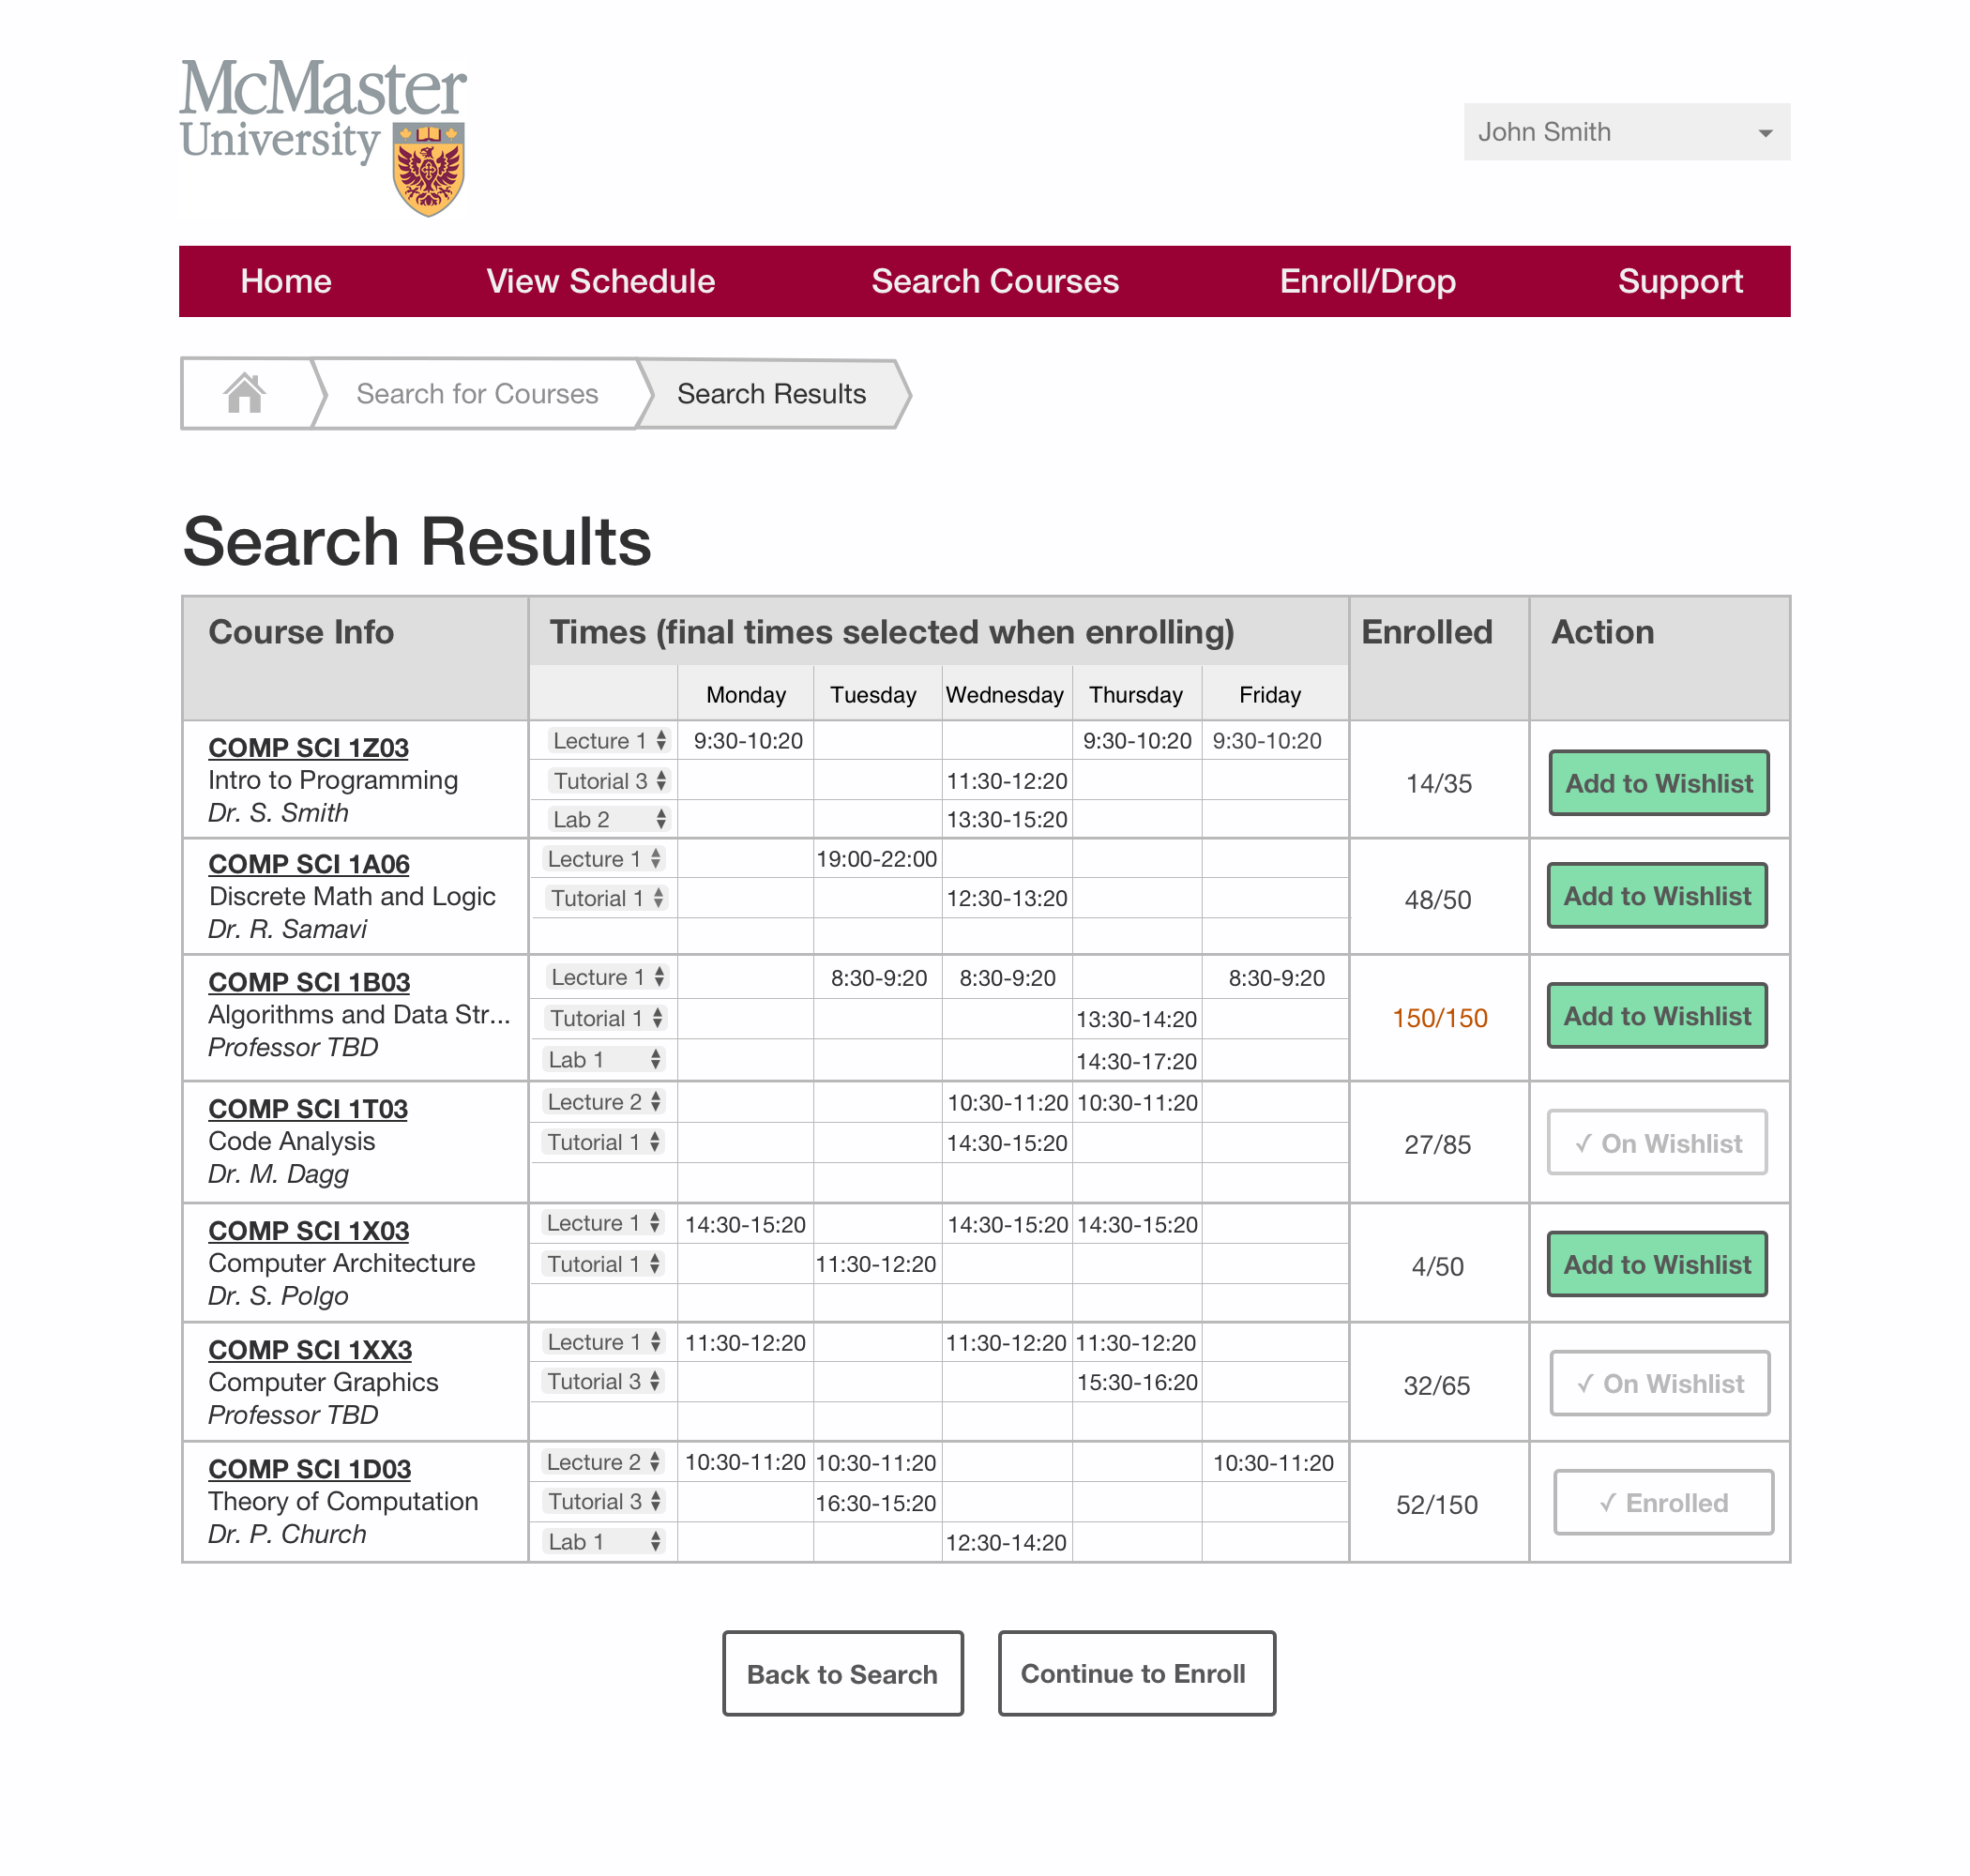
\includegraphics[height=80mm]{images/Rev2_CourseListing.png}}\\
%    \Caption{Final Mockup of Search Results Page}
%\end{minipage}
%\begin{minipage}{.5\textwidth}
%    \centering
%    \fbox{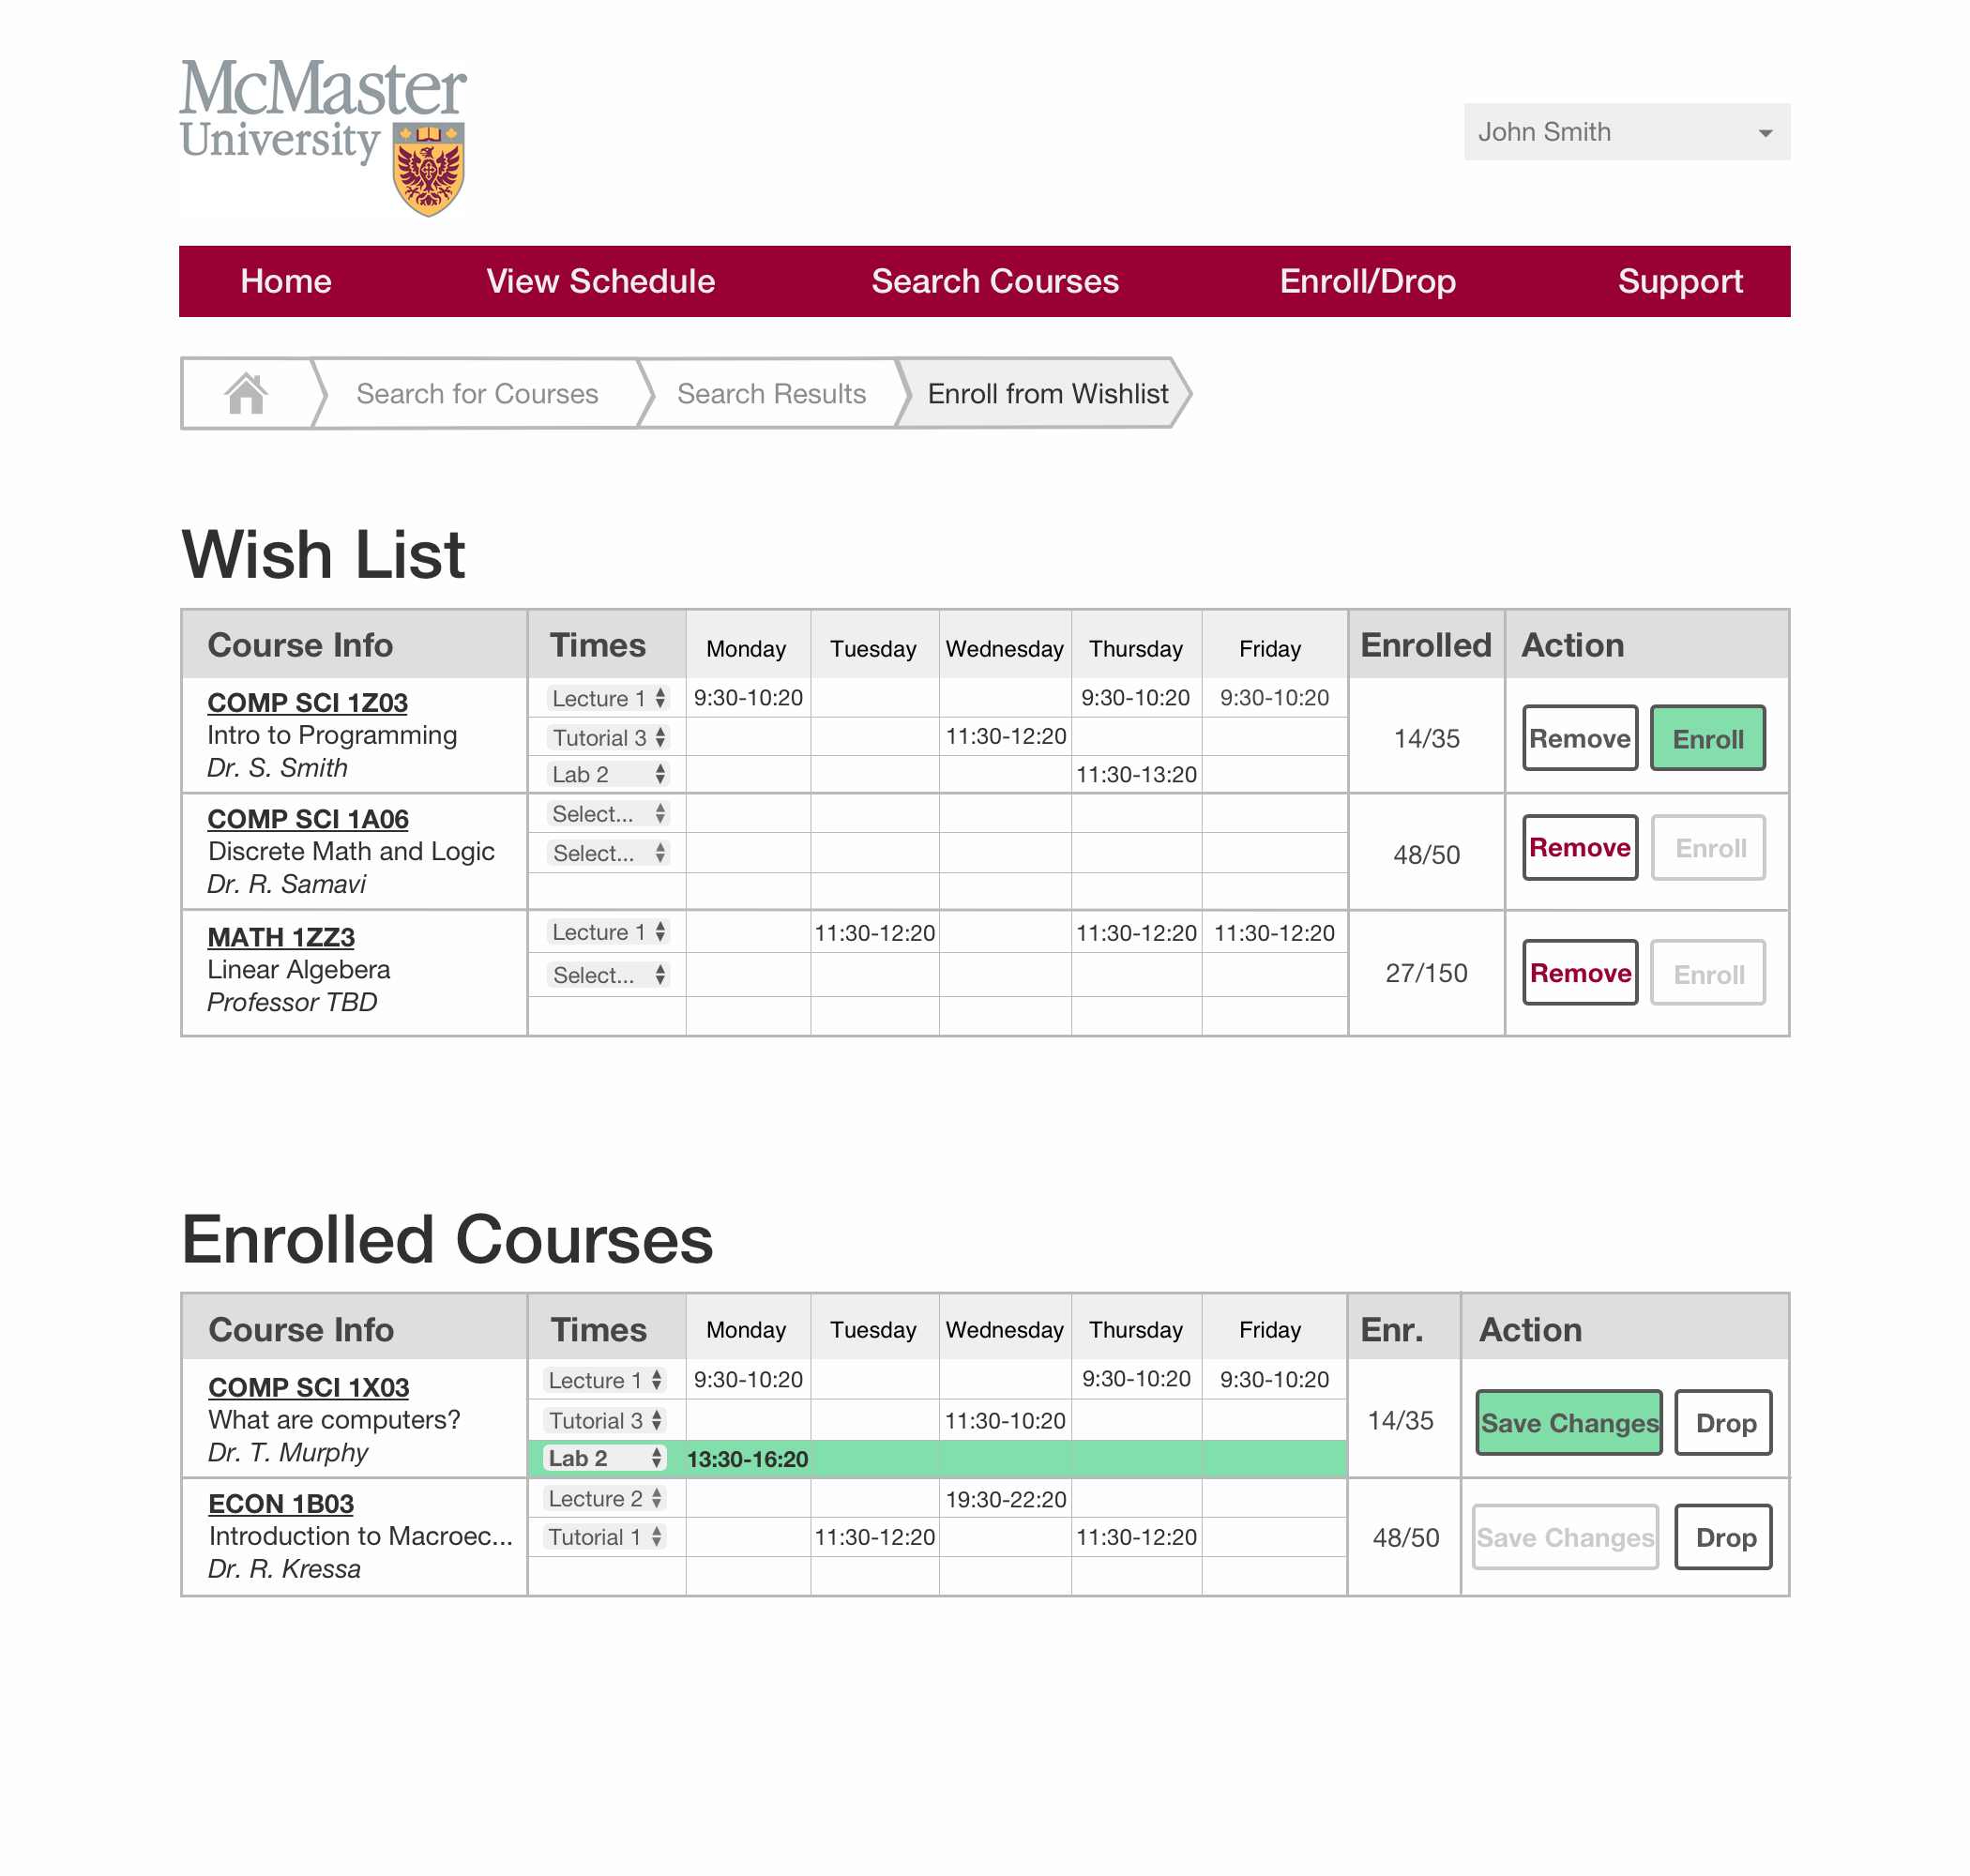
\includegraphics[height=80mm]{images/Rev2_WishlistEnroll.png}}\\
%    \Caption{Final Mockup of Enroll from Wishlist Page}
%\end{minipage}\\\vspace{5mm}
%
%% ================== SUBSECTION ============================ %
%\subsection*{New System -- HTA's}
%\begin{figure}[h]
%\centering
%\fbox{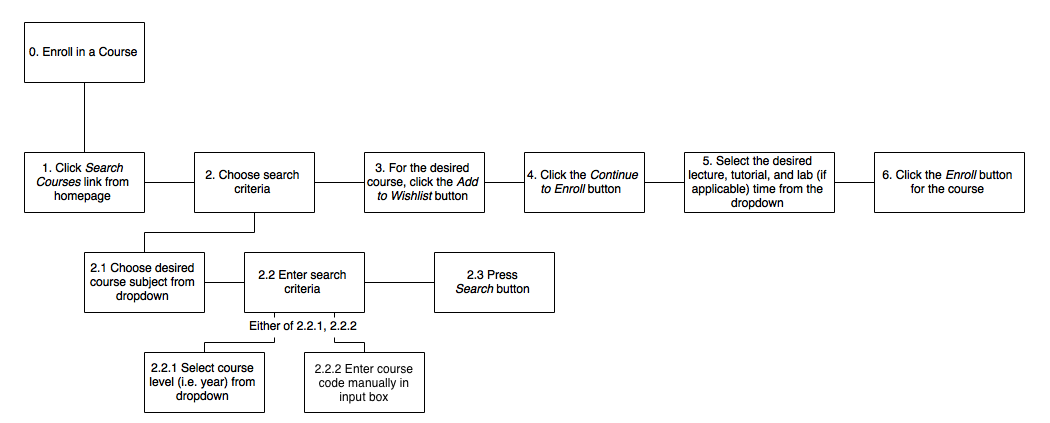
\includegraphics[width=\textwidth]{images/HTA_Enroll.png}}\\
%\Caption{New System HTA - Enrolling in a Course}
%\end{figure}
%
%\begin{figure}[h]
%\centering
%\fbox{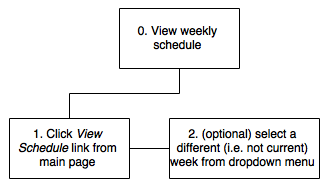
\includegraphics[width=60mm]{images/HTA_ViewSchedule.png}}\\
%\Caption{New System HTA - View Weekly Schedule}
%\end{figure}
%
%% ================== SUBSECTION ============================ %
%\subsection*{New System -- Screenshots}
%\begin{figure}[h]
%    \centering
%    \fbox{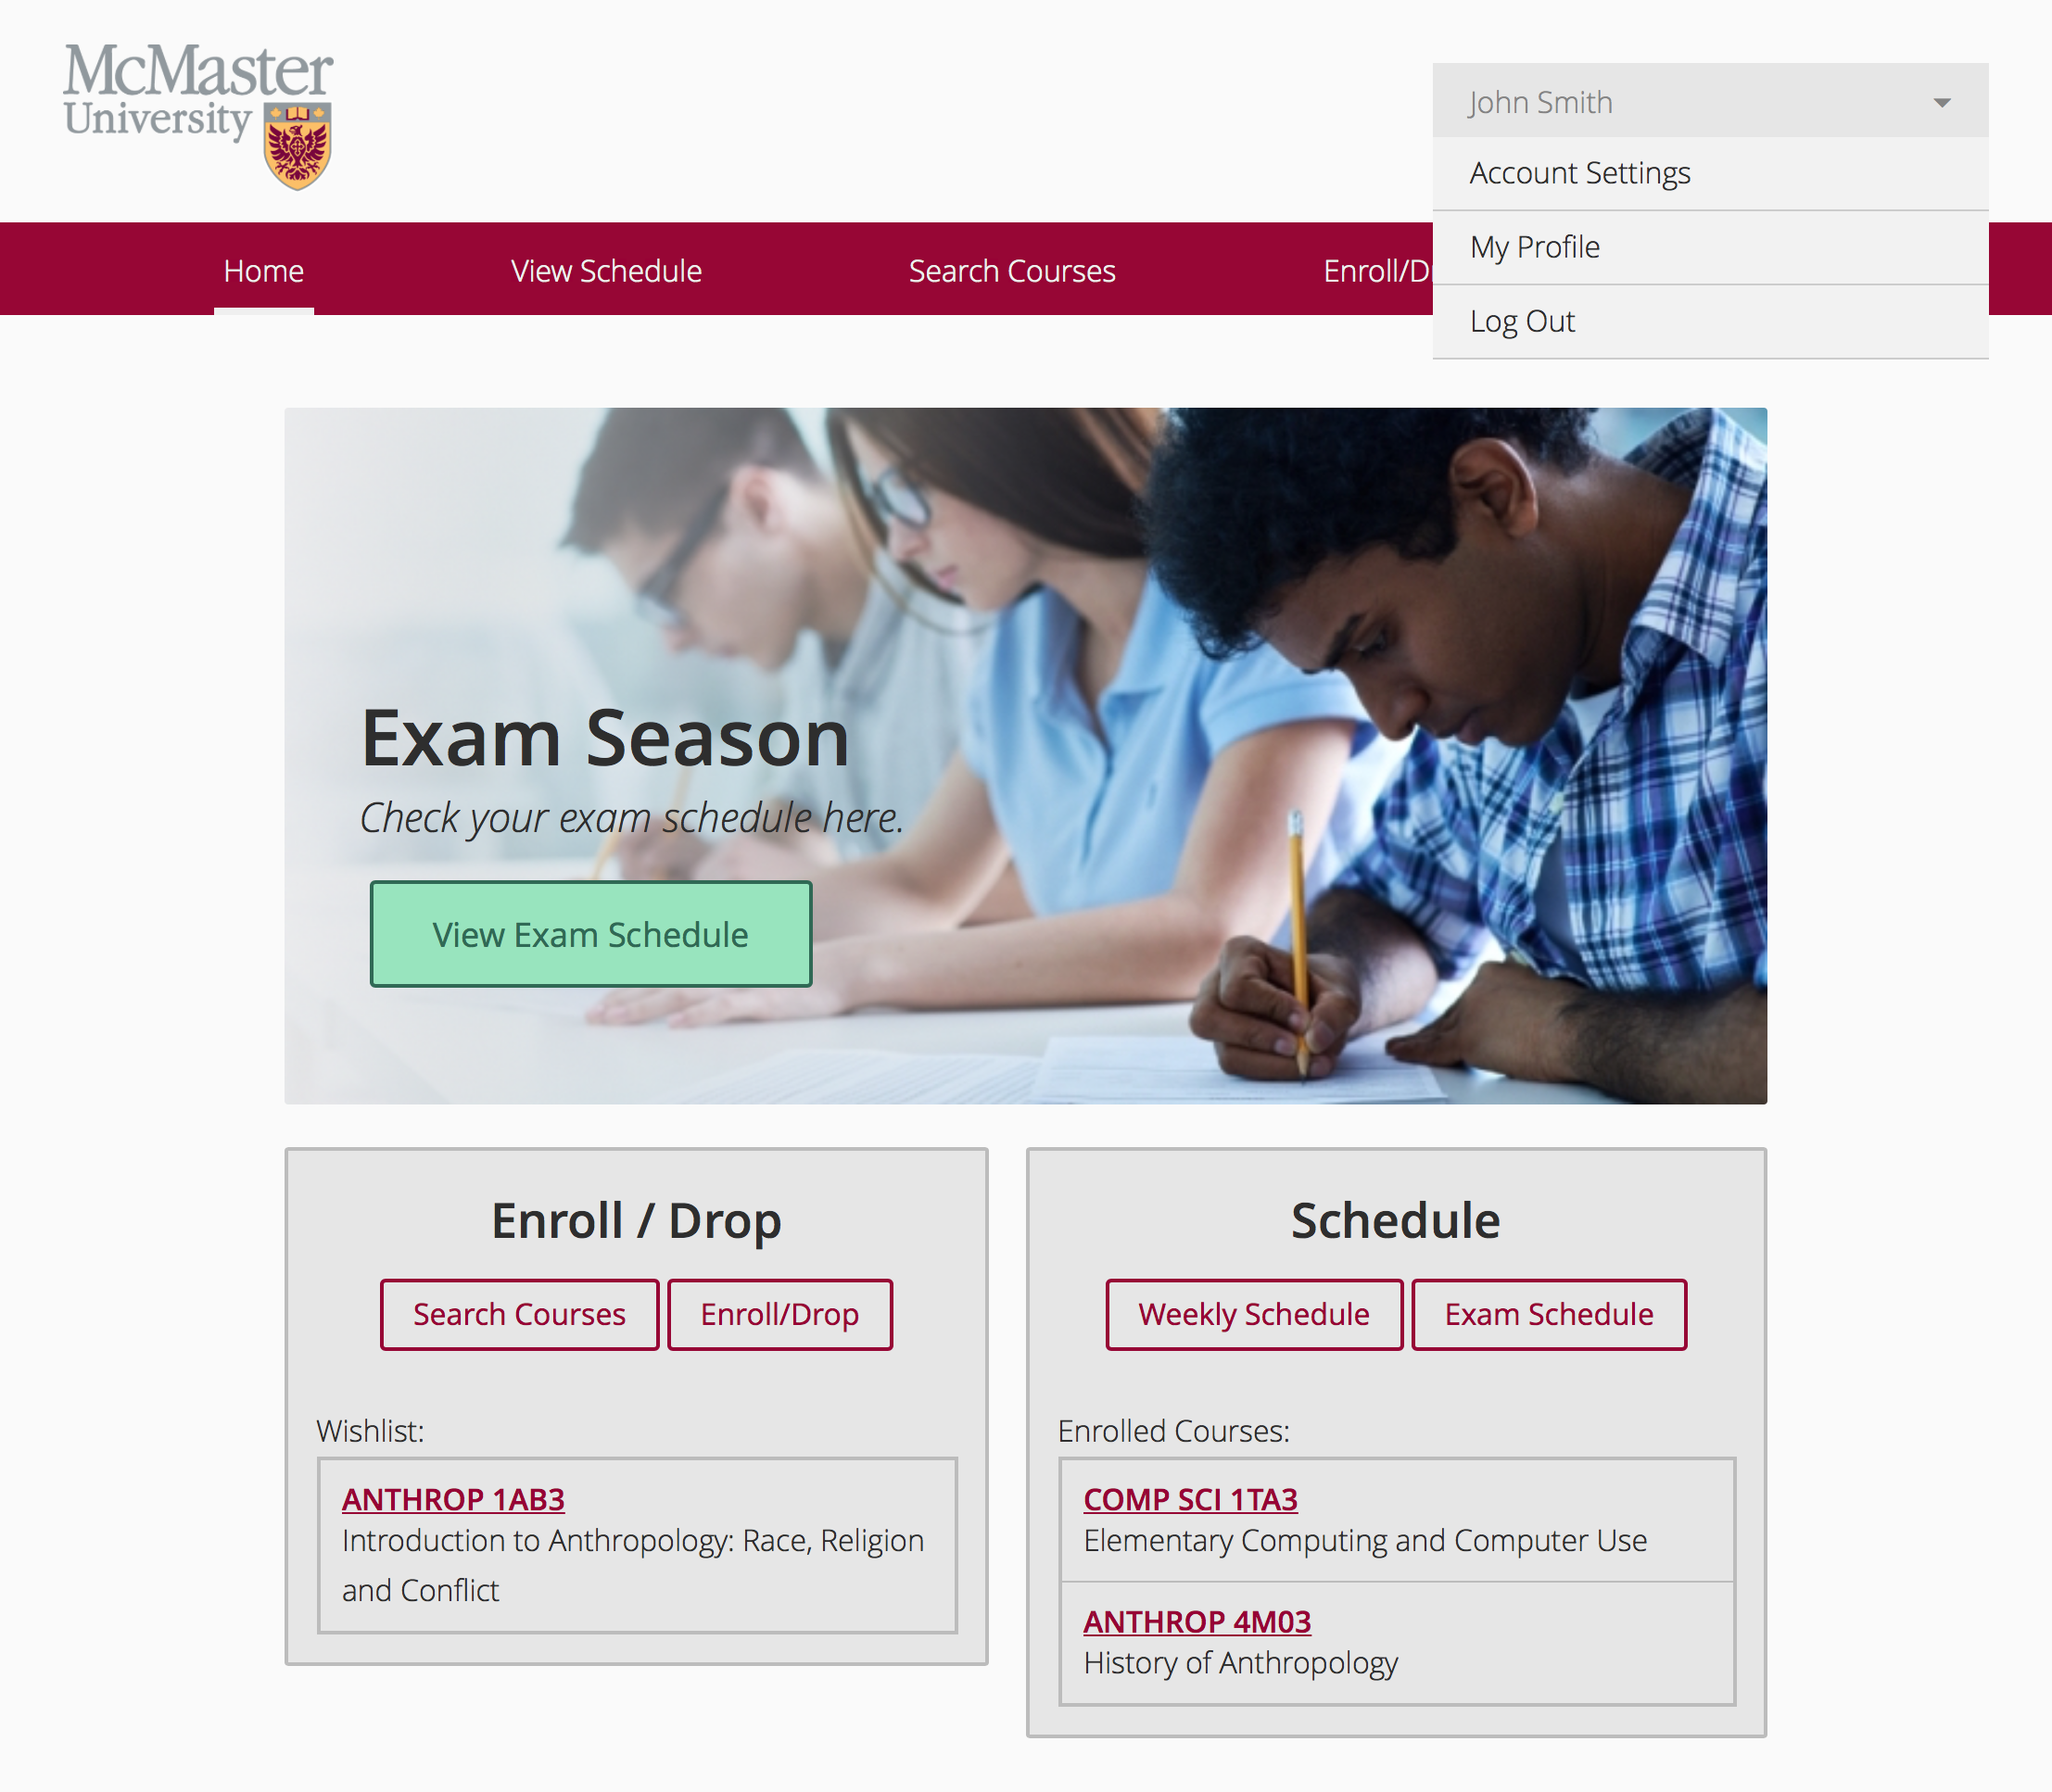
\includegraphics[width=\textwidth]{images/screen_home.png}}\\
%    \Caption{New System Screenshot -- Home Page}
%\end{figure}
%\begin{figure}[h]
%    \centering
%    \fbox{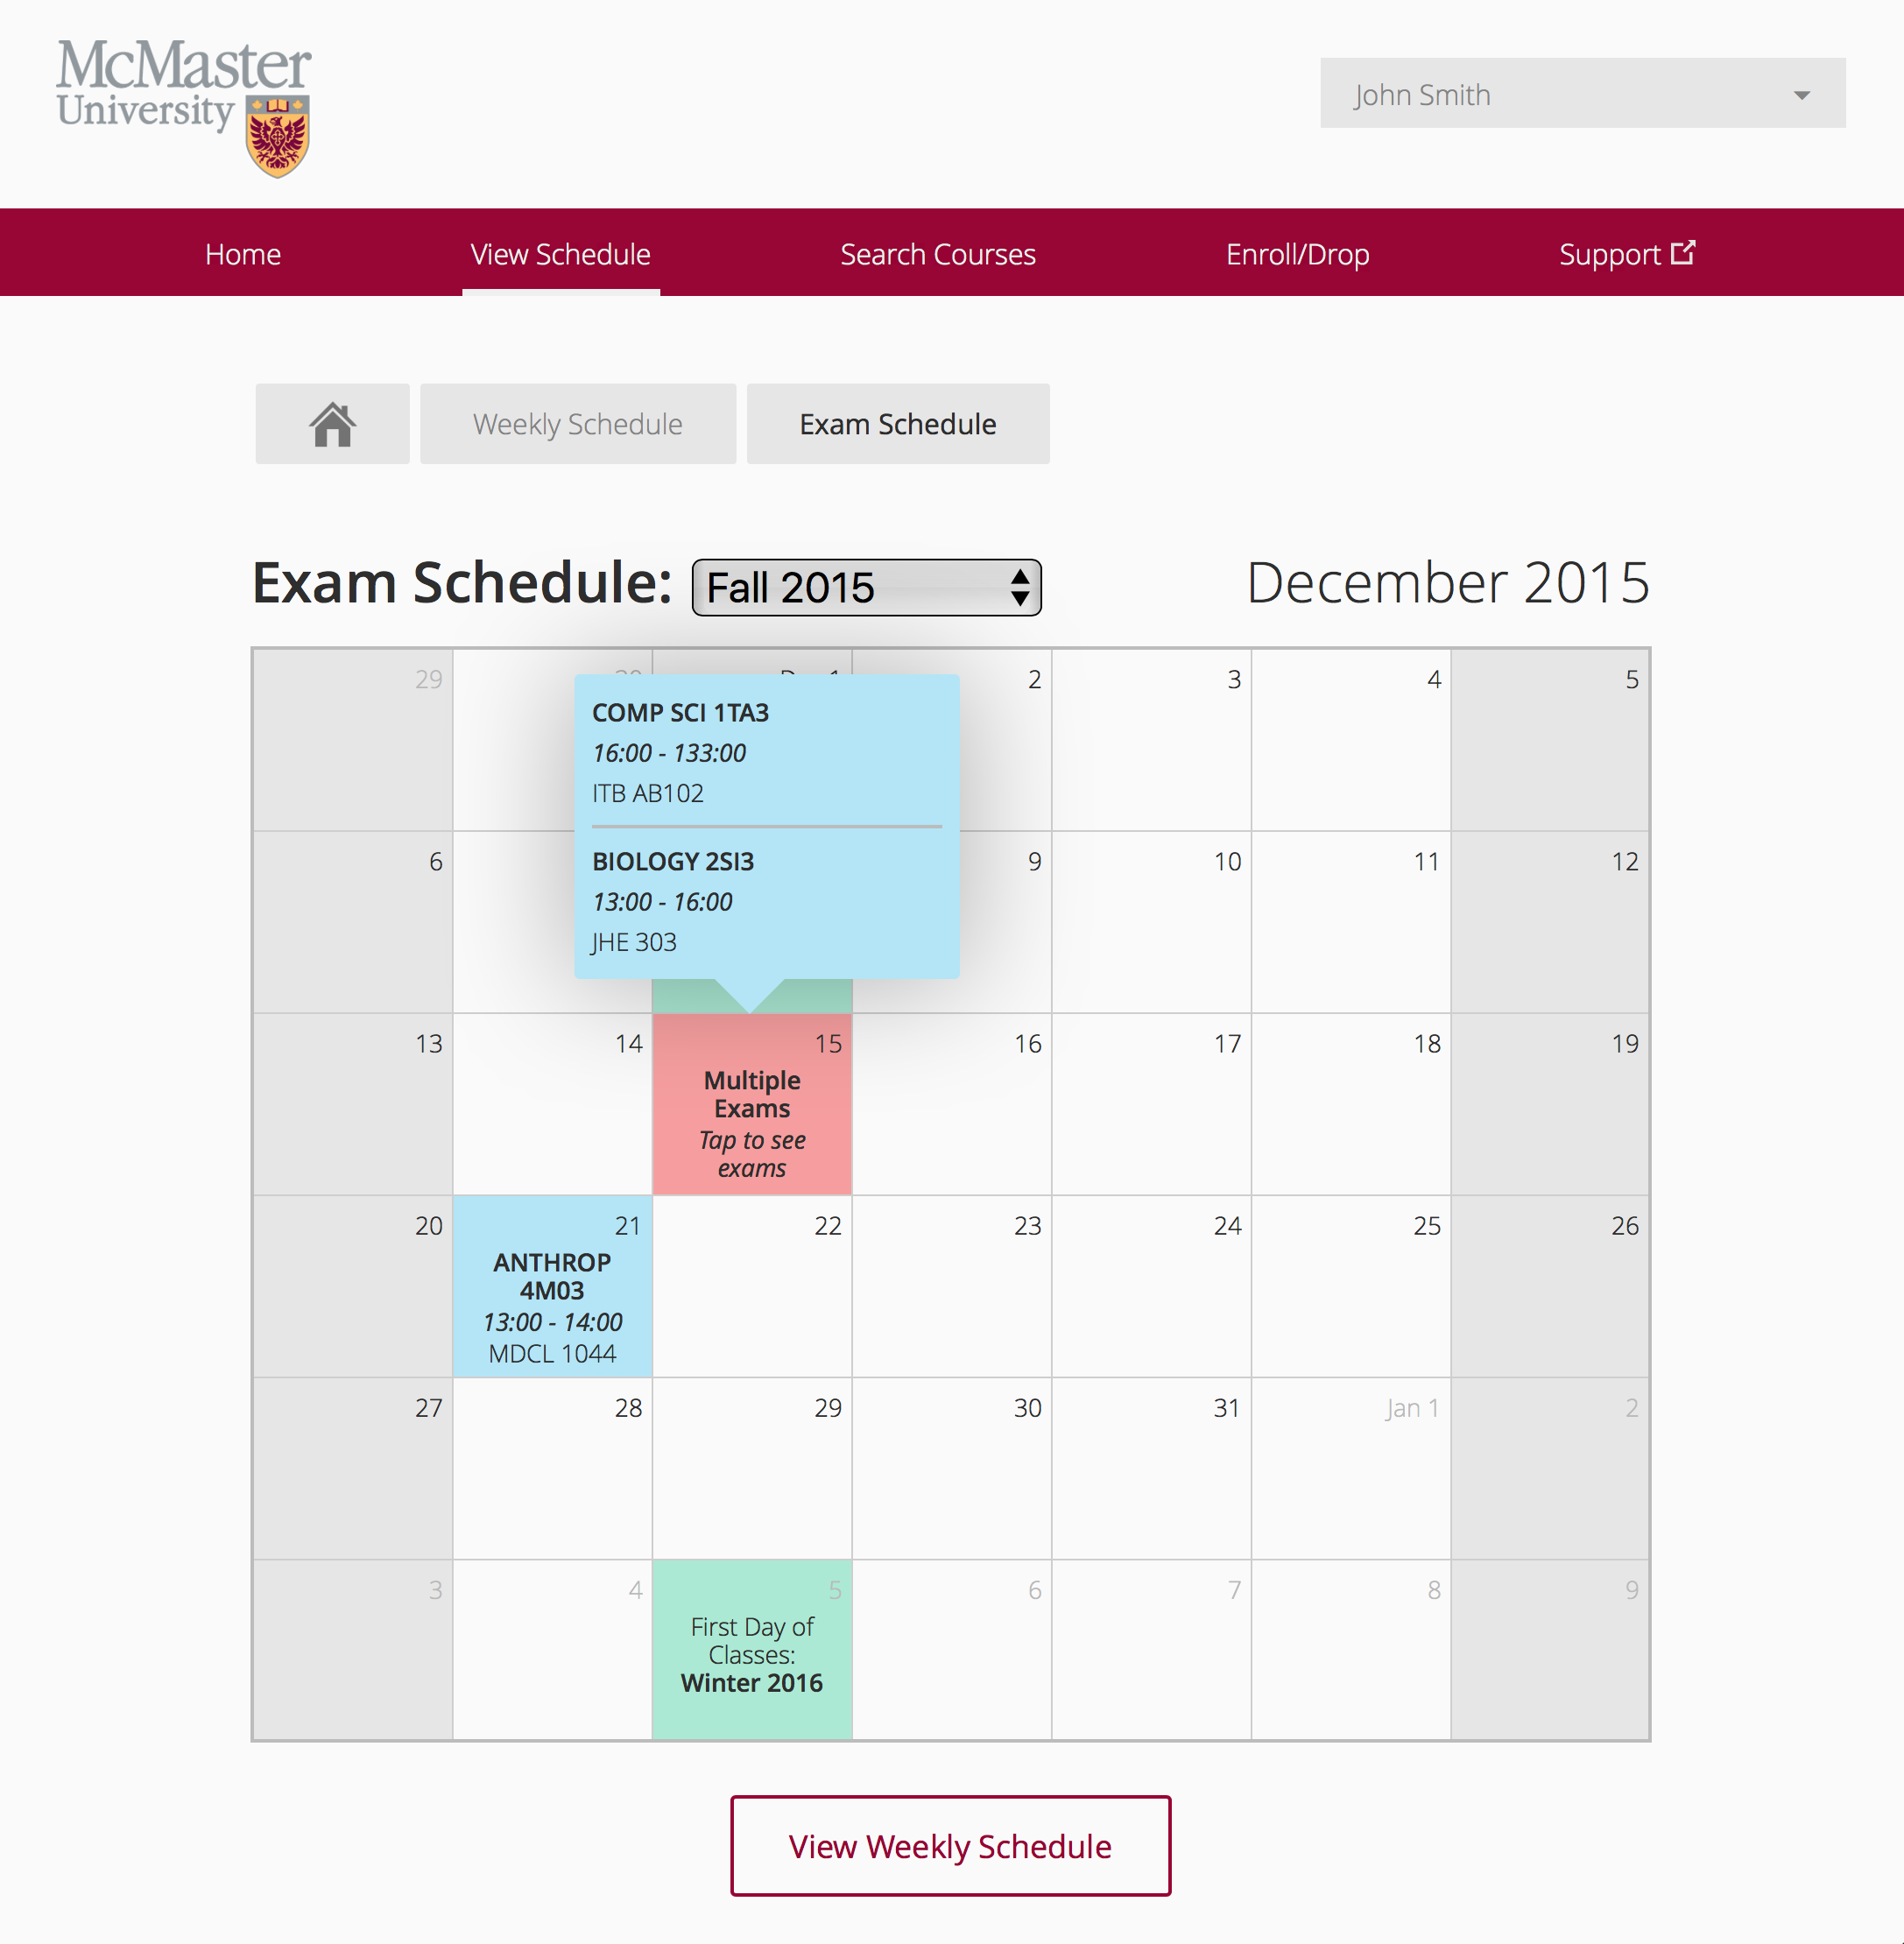
\includegraphics[width=\textwidth]{images/screen_exam.png}}\\
%    \Caption{New System Screenshot --  Exam Schedule}
%\end{figure}
%
%\begin{figure}[h]
%    \centering
%    \fbox{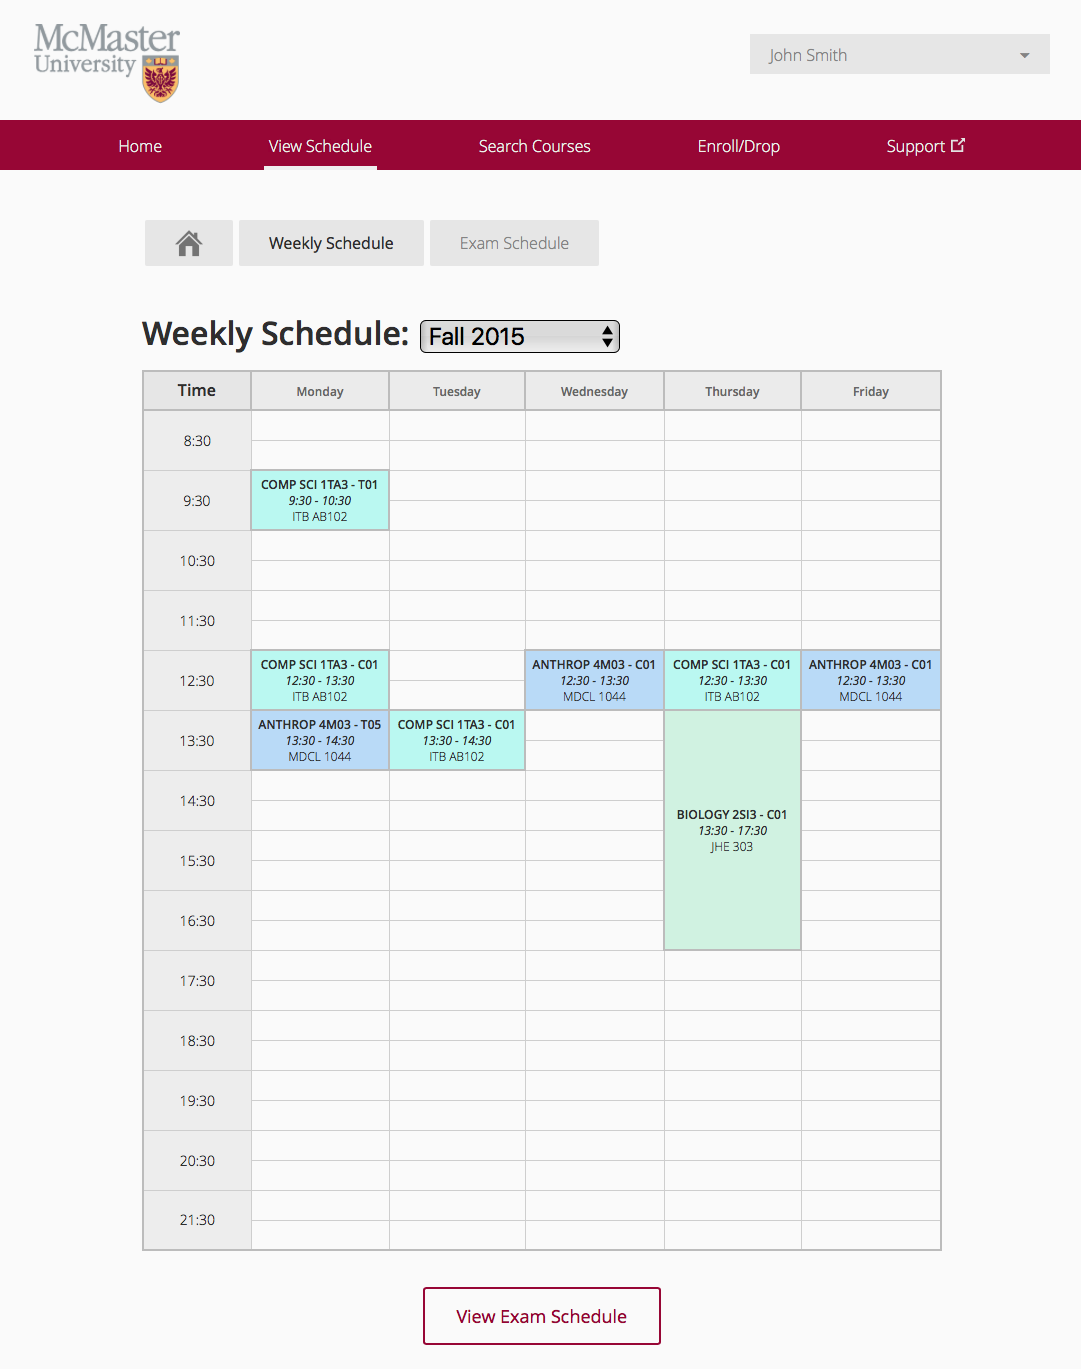
\includegraphics[width=\textwidth]{images/screen_weekly.png}}\\
%	\Caption{New System Screenshot -- Weekly Schedule}
%\end{figure}
%
%\begin{figure}
%    \centering
%	\fbox{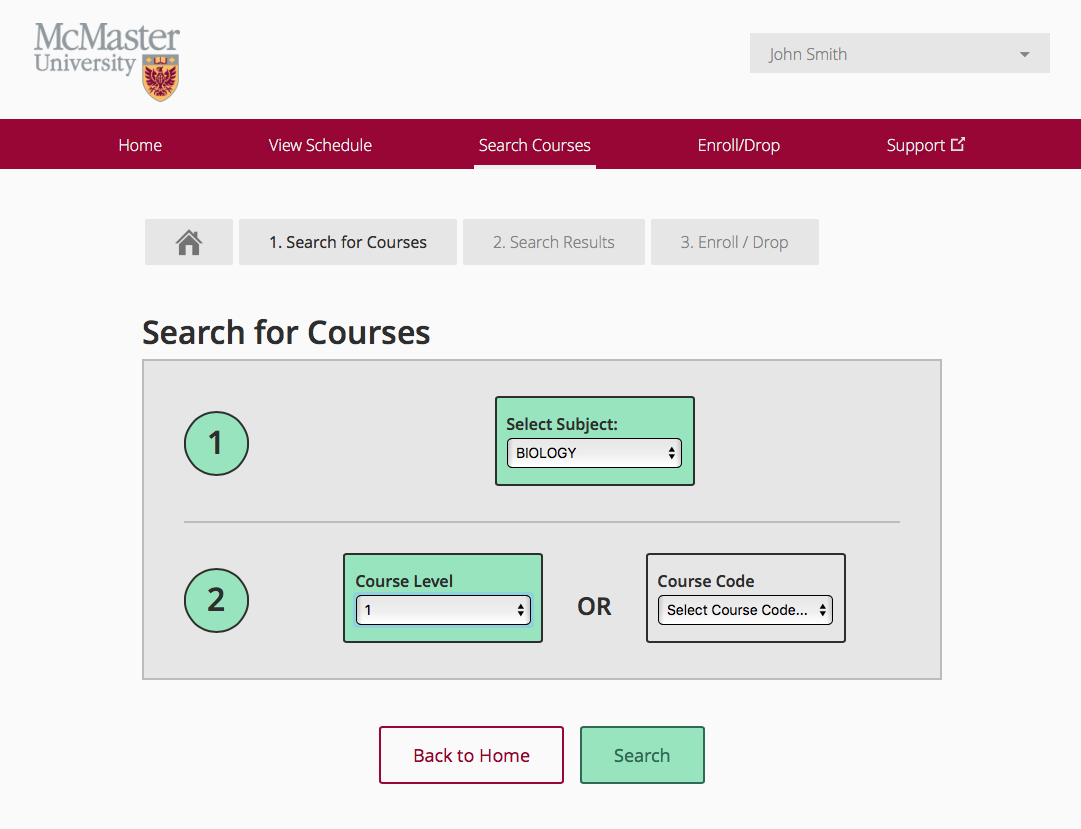
\includegraphics[width=\textwidth]{images/screen_criteria.png}}\\
%	\Caption{New System Screenshot -- Search Criteria Page}
%\end{figure}
%
%\begin{figure}
%    \centering
%    \fbox{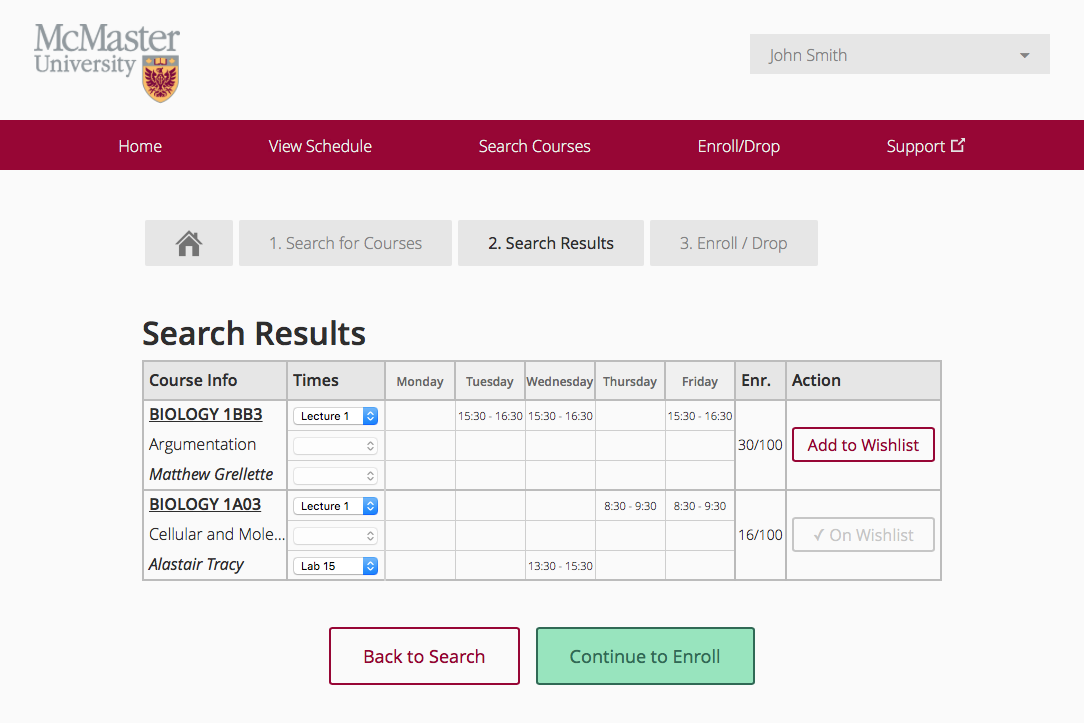
\includegraphics[width=\textwidth]{images/screen_results.png}}\\
%    \Caption{New System Screenshot -- Search Results Page}
%\end{figure}
%
%\begin{figure}[h]
%    \centering
%    \fbox{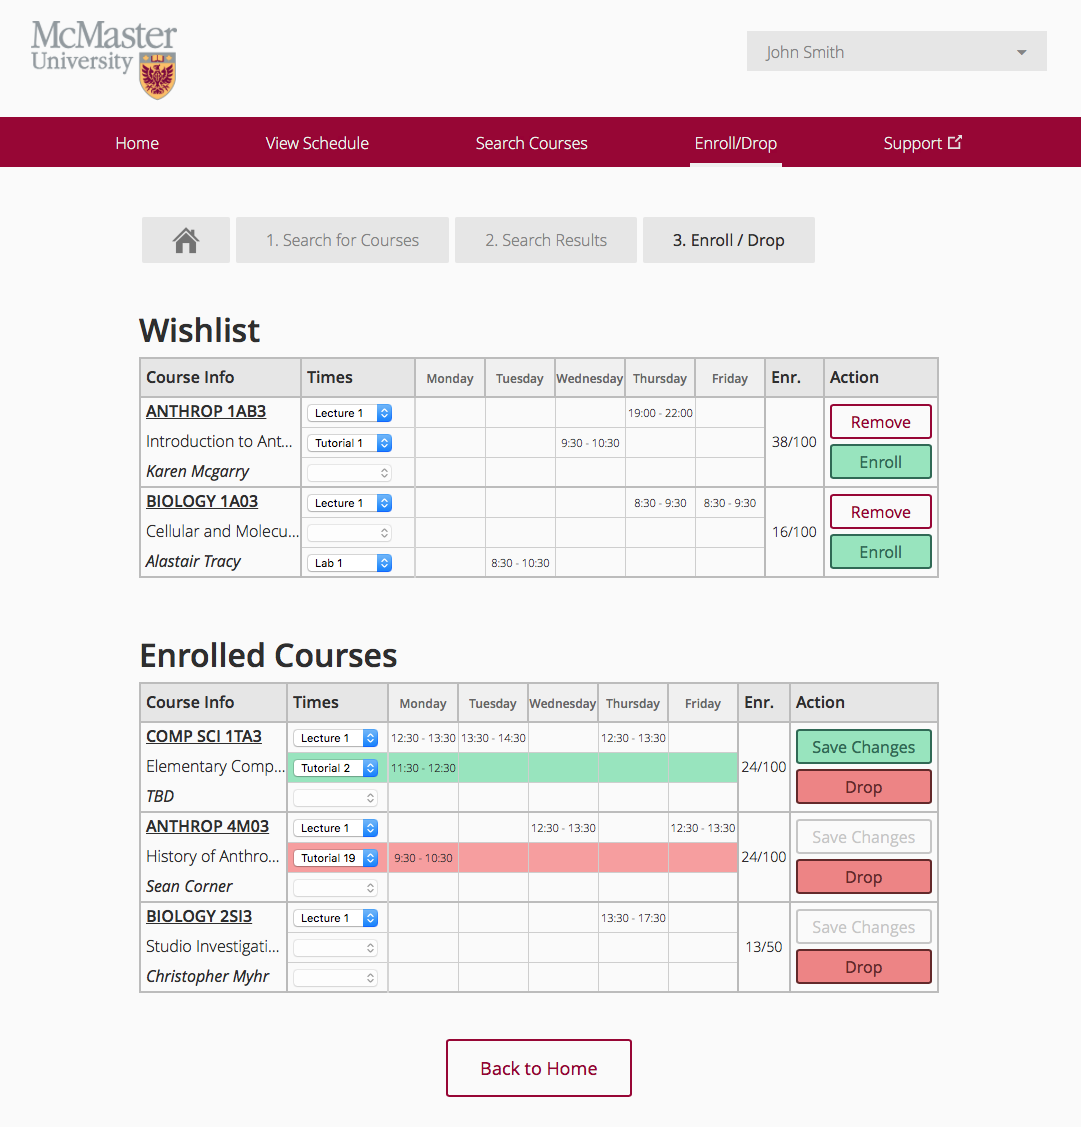
\includegraphics[width=\textwidth]{images/screen_enroll.png}}\\
%    \Caption{New System Screenshot --  Enroll from Wishlist Page}
%\end{figure}
%

\end{document}
